% !TEX encoding = UTF-8 Unicode
% !TEX TS-program = pdflatex
% !TEX spellcheck = it-IT

\documentclass{beamer}
\usepackage[T1]{fontenc}
\usepackage[utf8]{inputenc}
\usepackage[italian]{babel}
%\usepackage{amsmath}
%\usepackage{amssymb}
\usepackage {amsfonts, amsmath, amssymb, esint, mathrsfs}
\usepackage{amsthm}
\usepackage{mathtools}
\usepackage{braket}
\usepackage{bm}
\usepackage{bbm}

\usepackage {booktabs}									%tabelle
\usepackage {multirow}

\usepackage {graphicx}									%Immagini
\usepackage {subfigure}

\title[Controllo ottimo parabolico]{Strategie e analisi dell'errore per problemi di ottimizzazione vincolati regolati da equazioni di evoluzione}
\author[Arbib \& Bonomi]{Claudia Bonomi  Edoardo Arbib}
\date[Progetto anedp]{Progetto per il corso di Analisi Numerica per le Equazioni a Derivate Parziali II}
\institute[Polimi]{POLITECNICO DI MILANO}
%\logo{img/polimiLogo}

%\usetheme{AnnArbor}
%\useoutertheme[right]{sidebar}

  \usetheme{Darmstadt}
%  \usetheme{Boadilla}
%  \usecolortheme{seahorse}
 % \usecolortheme{rose}
 \usecolortheme{crane}


\setbeamercovered{dynamic}

%\theoremstyle{plain}
%\newtheorem{lemma}{Lemma}
\theoremstyle{definition}
\newtheorem{definizione}{Definizione}
\theoremstyle{remark}
\newtheorem{osservazione}{Osservazione}
\theoremstyle{plain}
\newtheorem{teorema}{Teorema}
\theoremstyle{definition}
\newtheorem{algoritmo}{Algoritmo}

\DeclarePairedDelimiter{\abs}{\lvert}{\rvert}
\DeclarePairedDelimiter{\norma}{\lVert}{\rVert}

\DeclareMathOperator{\argmin}{arg\,min}

\newcommand{\numberset}{\mathbb}
\newcommand{\N}{\numberset{N}}
\newcommand{\R}{\numberset{R}}
\newcommand{\Z}{\numberset{Z}}


\begin{document}

\begin{frame}
\maketitle
\end{frame}

\begin{frame}
\frametitle{Contenuti}
\tableofcontents
\end{frame}


\section{Problema continuo}
\begin{frame}
\frametitle{Setting}
dominio $ \Omega\times I,\  \Omega \subset \mathbb{R}^n,\ I=(0,T),\ U_{ad}\subset U=L^2(I,\R^D) $ 
\begin{equation}
%\tag{$\mathbb{P}$}
\begin{aligned}
& \underset{y \in Y, u \in U_{ad}}{\text{min}}
& & J(y,u) = \frac{1}{2}{||y-y_d||^{2}}_{L^2(I,{L^{2}(\Omega)})} + \frac{\alpha}{2}{||u||^{2}}_U \\
& \text{s.t.} & & y = S(Bu,y_0) \\
%\label{eq:200}
\end{aligned}
\end{equation}

\begin{columns}[t]
\begin{column}{0.4\textwidth}
Equazione di stato
\begin{equation*}
\begin{array}{cc}
 	{\partial_{t}}\overline{y} - {\bigtriangleup}\overline{y} = f & \text{in I}\times\Omega \\
	\overline{y}=0 & \text{in I}\times\Omega \\
	\overline{y}(0) = \kappa & \text{in }\Omega \\
\end{array}
%\label{eq:201}
\end{equation*}
\end{column}

\begin{column}{0.4\textwidth}
Condizione di ottimalità 
\begin{equation*}
\overline{u}=P_{U_{ad}}\left( -\frac{1}{\alpha}B'\overline{p} \right)
%\label{eq:213}
\end{equation*}
\end{column}
\end{columns}

$\overline{p} $ è la soluzione del problema aggiunto
\begin{equation}
\begin{aligned}
& -{\partial_{t}}\overline{p} -\bigtriangleup\overline{p} =\overline{y} - y_d & & \text{in }I{\times}\Omega \\
& \overline{p}=0 & & \text{in }I{\times}\partial\Omega \\
& \overline{p}(T)=0 & & \text{su }\Omega \\
\label{eq:217}
\end{aligned}
\end{equation}
\end{frame}

\begin{frame}
\frametitle{Spazio e operatore di controllo}
Spazio di controllo
\begin{equation}
U_{ad} = \left\{ u \in U | a_i \leq u_i(t) \leq b_i {\forall}i=1:d  \right\}
\label{eq:208}
\end{equation}
con $a_i, b_i \in \mathbb{R}$ t.c. $a_i<b_i \ {\forall}i=1:d$


Operatore di controllo
\begin{equation}
B : U \rightarrow L^2(I,{H^{-1}(\Omega)}),\ u\mapsto \left( t\mapsto\sum_{i=1}^d u_i(t)g_i \right)
\label{eq:209}
\end{equation}
con funzionali noti $g_i \in {H^{-1}(\Omega)}$
\end{frame}


\section{Problema discreto}
\subsection{Equazioni di stato e aggiunta}
\begin{frame}
\frametitle{Discretizzazione temporale}
Partizione di $[0,T)$ in sottointervalli $I_m=[t_{m-1},t_m)$, dove $0=t_0<t_1<\dots<t_M=T\ \longrightarrow $ griglia primale

 Seconda partizione di $ [0,T) $ in intervalli $I^*_m=[t^*_{m-1},t^*_m)$, con $0=t^*_0<t^*_1<\dots<t^*_M=T$ e $t^*_m=\frac{t_{m-1}+t_m}{2}\quad\text{per $m=1,\dots,M$} \ \longrightarrow $ griglia duale
 
 Ambientazione funzionale
 \begin{gather*}
P_k:=\Bigl\{v\in C([0,T],H^1_0(\Omega))\Bigl| v|_{I_{m}}\in \mathcal{P}_1(I_m,H^1_0(\Omega))\Bigr\},\\
P^*_k:=\Bigl\{v\in C([0,T],H^1_0(\Omega))\Bigl| v|_{I^*_{m}}\in \mathcal{P}_1(I^*_m,H^1_0(\Omega))\Bigr\},\\  
  Y_k:=\Bigl\{v:[0,T]\to H^1_0(\Omega)\Bigl| v|_{I_{m}}\in \mathcal{P}_0(I_m,H^1_0(\Omega))\Bigr\}.
\end{gather*}
\end{frame}

\begin{frame}
\frametitle{Operatori di interpolazione}
\begin{enumerate}[<+->]
\item $\mathcal{P}_{Y_{k}}:L^2(I,H^1_0(\Omega))\to Y_k$
\[
\mathcal{P}_{Y_{k}} v|_{I_{m}}:=\frac{1}{k_{m}} \int^{t_{m}}_{t_{m-1}}vdt \ \text{for $m=1,\dots,M$}, \ \text{e}\ \mathcal{P}_{Y_{k}}v(T):=0
\]
\item $\Pi_{Y_{k}}:C([0,T],H^1_0(\Omega))\to Y_k$
\[
\Pi_{Y_{k}} v|_{I_{m}}:=v(t^*_m)\quad\text{per $m=1,\dots,M$},\quad \Pi_{Y_{k}} v(T):=v(T)
\]
\item $\pi_{P^*_k}:C([0,T],H^1_0(\Omega))\cup Y_k\to P^*_k$
\begin{gather*}
\pi_{P^*_k} v|_{I^*_1\cup I^*_2}:=v(t^*_1)+\frac{t-t^*_1}{t^*_2-t^*_1}(v(t^*_2)-v(t^*_1)),\\
\pi_{P^*_k} v|_{I^*_m}:=v(t^*_{m-1})+\frac{t-t^*_{m-1}}{t^*_{m}-t^*_{m-1}}(v(t^*_m)-v(t^*_{m-1})),\\
\pi_{P^*_k} v|_{I^*_M\cup I^*_{M+1}}:=v(t^*_{M-1})+\frac{t-t^*_{M-1}}{t^*_M-t^*_{M-1}}(v(t^*_M)-v(t^*_{M-1})).
\end{gather*}
\end{enumerate} 
\end{frame}

\begin{frame}
\frametitle{Equazione di stato}
Formulazione debole
trovare $y_k\in Y_k$ tale che 
\begin{multline}
%\label{eqn:stato}
 \int_{0}^{T}\!\!\!\!\! -\left \langle {\partial_{t}}v(t),y(t) \right \rangle_{{H^{-1}}{H^{1}_{0}}} dt + \int_{0}^{T}\!\!\!\!\! a(y(t),v(t)) dt + (y(T),v(T))_{L^{2}} \\
=\int^{T}_{0} \Braket{f(t),v_k(t)}_{H^{-1}H^1_0}dt + (\kappa,v_k(0))_{L^2}\ \forall v_k\in P_k.
\end{multline}
$ \Rightarrow $ variante di CN con passo di Rannacher. Lo schema è consistente, stabile, convergente.
\begin{block}{Analisi errore}
$y_k\in Y_k\Rightarrow$  ordine $\mathcal{O}(k)$, ma $ \pi_{P^*_k}y_k $ converge con ordine due
\end{block}
Lo studio dell'equazione aggiunta è analogo, solo con spazi di soluzione e test scambiati. Lo schema risultante è una variante di CN.
\end{frame}


\subsection{Discretizzazione variazionale}
\begin{frame}
\frametitle{Discretizzazione variazionale}
Problema di controllo ottimo discretizzato
\begin{equation}
\tag{$\mathbb{P}_k$}
\begin{aligned}
& \underset{y_k \in Y_k, u \in U_{ad}}{\text{min}}
& & J(y_k,u) = \frac{1}{2}\norma{y_k-y_d}^2_{L^2(I,L^2(\Omega))} + \frac{\alpha}{2}\norma{u}^2_U \\
& \text{s.t.} & & y_k = S_k(Bu,y_0) 
\label{Pk}
\end{aligned}
\end{equation}
dove $ S_k $ è la discretizzazione di $ S $ tramite lo schema di PG.
\begin{block}{Osservazioni}
\begin{enumerate}[<+->]
\item Il metodo si basa sulla discretizzazione dei soli spazi di stato e aggiunto, utilizzando implicitamente le condizioni di ottimalità del primo ordine per la discretizzazione del controllo.
\item Il metodo permette di disaccoppiare l'approssimazione dell'\textit{active set} dalla scelta della griglia temporale
\item Il metodo è ben posto e convergente con ordine $ 2 $ rispetto al controllo $ u $.
\end{enumerate}
\end{block}
\end{frame}

\section{Algoritmi risolutivi}
\begin{frame}
\frametitle{Punto fisso}
La CNES di ottimalità del problema discreto è sempre $ \bar{u}_k=P_{U_{ad}}\big( -\frac{1}{\alpha}B'\bar{p}_k\big) $. Le iterazioni di punto fisso si applicano proprio a quest'equazione $ \Rightarrow $
\begin{block}{Algoritmo}
\begin{enumerate}
\item Inizializzare $ u^0_h\in U_{ad} $, $ n:=0 $.
\item Ripetere fino a convergenza
          \begin{enumerate}
          \item calcolare $ Bu^n_h $,
          \item calcolare $ y^n_h=S_h(y_0,Bu^n_h) $, 
          \item calcolare $ p^n_h=S^*_h(y^n_h-y_d) $,
          \item calcolare $ u^{n+1}_h=P_{U_{ad}}\big( -\frac{1}{\alpha}B'p^n_h\big) $,
          \item porre n=n+1.
          \end{enumerate}
\end{enumerate}
Criterio di arresto: $ \norma{B'\big(p^{n+1}_h-p^n_h\big)}_{L^{\infty}(\Omega\times I)}<\epsilon $
\end{block}
{\scshape {\Large Non converge per $ \alpha $ piccoli}}
\end{frame}

\begin{frame}
\frametitle{Semi-Newton}
Metodo di Newton con minimizzazione monodimensionale (Armijo) $ \Rightarrow $ formulazione del problema tramite Lagrangiana primale e duale
\begin{multline}
%\label{lagr}
\phi(w)= \\
-\inf_{u,y\in L^2(I,L^2)}\Biggl( \underbrace{\frac{1}{2}\norma{y-y_d}^2 + \frac{\alpha}{2}\norma{u}^2  + \chi_{U_{ad}}(u) - (w,y-S_hu)}_{\mathcal{L}(u,y,w)}\Biggr)
\end{multline}
che diventa quindi un caso di minimizzazione non vincolata $ \min_{w\in L^2(I,L^2(\Omega))} \phi(w) $.
%Qual è la CNES di ottimalità? Si può applicare un metodo di Newton? Risponde il seguente
\end{frame}

\begin{frame}
\frametitle{Semi-Newton II}
\begin{lemma}
%\label{phi}
La funzione $ \phi:L^2(I,L^2(\Omega))\to\R $  è fortemente convessa e Frechet-differenziabile con gradiente lipschitziano
\begin{equation}
\nabla\phi(w)=y(w)-S_hu(w),
\end{equation}
dove $ y_h(w)=w+y_d $ e $ u(w)=P_{U_{ad}}(-\frac{1}{\alpha}S^*_hw) $ sono gli unici punti di minimo della lagrangiana $ \mathcal{L}(u,y,w) $ per ogni $ w\in L^2(I,L^2(\Omega)) $ data.
\end{lemma}
Ma allora calcolato l'Hessiano generalizzato di $ \phi $, ogni iterazione di Newton risolve
\begin{equation}
\label{newton}
\big( I + \frac{1}{\alpha}S_h\mathbbm{1}_{S^*_hw}S^*_h\big)\delta w=-(w+y_d)+S_hP{U_{ad}}\big( -\frac{1}{\alpha}S^*_hw\big).
\end{equation}
%Ecco quindi l'algoritmo promesso
\end{frame}

\begin{frame}
\frametitle{Semi-Newton III}
\begin{algoritmo}
%\label{dn}
\begin{enumerate}
\item Inizializzare $ w^0\in L^2(I,L^2(\Omega)) $, $\beta\in(0,1) $, $ k=0 $, 
\item Ripetere fino a convergenza
          \begin{enumerate}
          \item Risolvere l'equazione ~\eqref{newton} per $ \delta w^k $ tramite CG,
          \item Porre $ \lambda:=1 $,
          \item Finché risulta vera la condizione $ \phi(w^k+\lambda\delta w^k) > \phi(w) + \frac{1}{3}\lambda(\nabla\phi(w^k),\delta w^k)_{L^2(I,L^2(\Omega))} $, porre $ \lambda:=\beta\lambda $,
          \item Porre $ w^{k+1}=w^k + \lambda\delta w^k $
         \item Porre $ k:=k+1 $.
          \end{enumerate}
\end{enumerate}
criterio di arresto:$ \norma{\nabla\phi(w^k)}\le t_0 $
\end{algoritmo}
L'algoritmo converge e il criterio di arresto è plausibile.
\end{frame}

\begin{frame}
\frametitle{Significato della simbologia}
\begin{block}{$ \chi_{U_{ad}} $}
Indica la funzione caratteristica dell'insieme $ U_{ad} $ nel senso dell'analisi convessa, ovvero
\begin{equation}
\chi_{U_{ad}}=
\begin{cases}
0,        &\text{su} \ U_{ad},\\
\infty   &\text{su} \ L^2(I,L^2(\Omega))\setminus U_{ad}.
\end{cases}
\end{equation}
\end{block}
\begin{block}{$ \mathbbm{1}_{p_h(v)} $}
Introdotto l'\textit{inactive set} della funzione $ p_h $ come l'insieme $ \mathcal{I}(p_h)=\Set{\omega\in \Omega\times [0,T] | \big( -\frac{1}{\alpha}p_h(v)\big)(\omega)\in (a(\omega),b(\omega))} $ e $ \mathbbm{1}_{\mathcal{I}(p_h)} $ come la funzione indicatrice di tale insieme
con $ \mathbbm{1}_{p_h(v)} $ si denota l'endomorfismo auto-aggiunto in $ L^2(I,L^2(\Omega)) $ dato dalla moltiplicazione puntuale con $ \mathbbm{1}_{\mathcal{I}(p_h)} $. 
\end{block}

\end{frame}

\section{Implementazione}
\begin{frame}
\frametitle{Implementazione}
Gli strumenti di sviluppo utilizzati sono \textbf{Freefem++} e \textbf{GitHub}.

Processo di raffinamento temporale al livello l: 
\begin{equation}
Nk = ( 2^l + 1 )
\label{Nk}
\end{equation}


\end{frame}
\frametitle{Implementazione: Funzione per il calcolo dell'Errore}
\begin{frame}

Per il calcolo di ogni norma e prodotto scalare il metodo numerico di integrazione in tempo utilizzato è il metodo di Cavalieri Simpson.

\begin{figure}
\centering
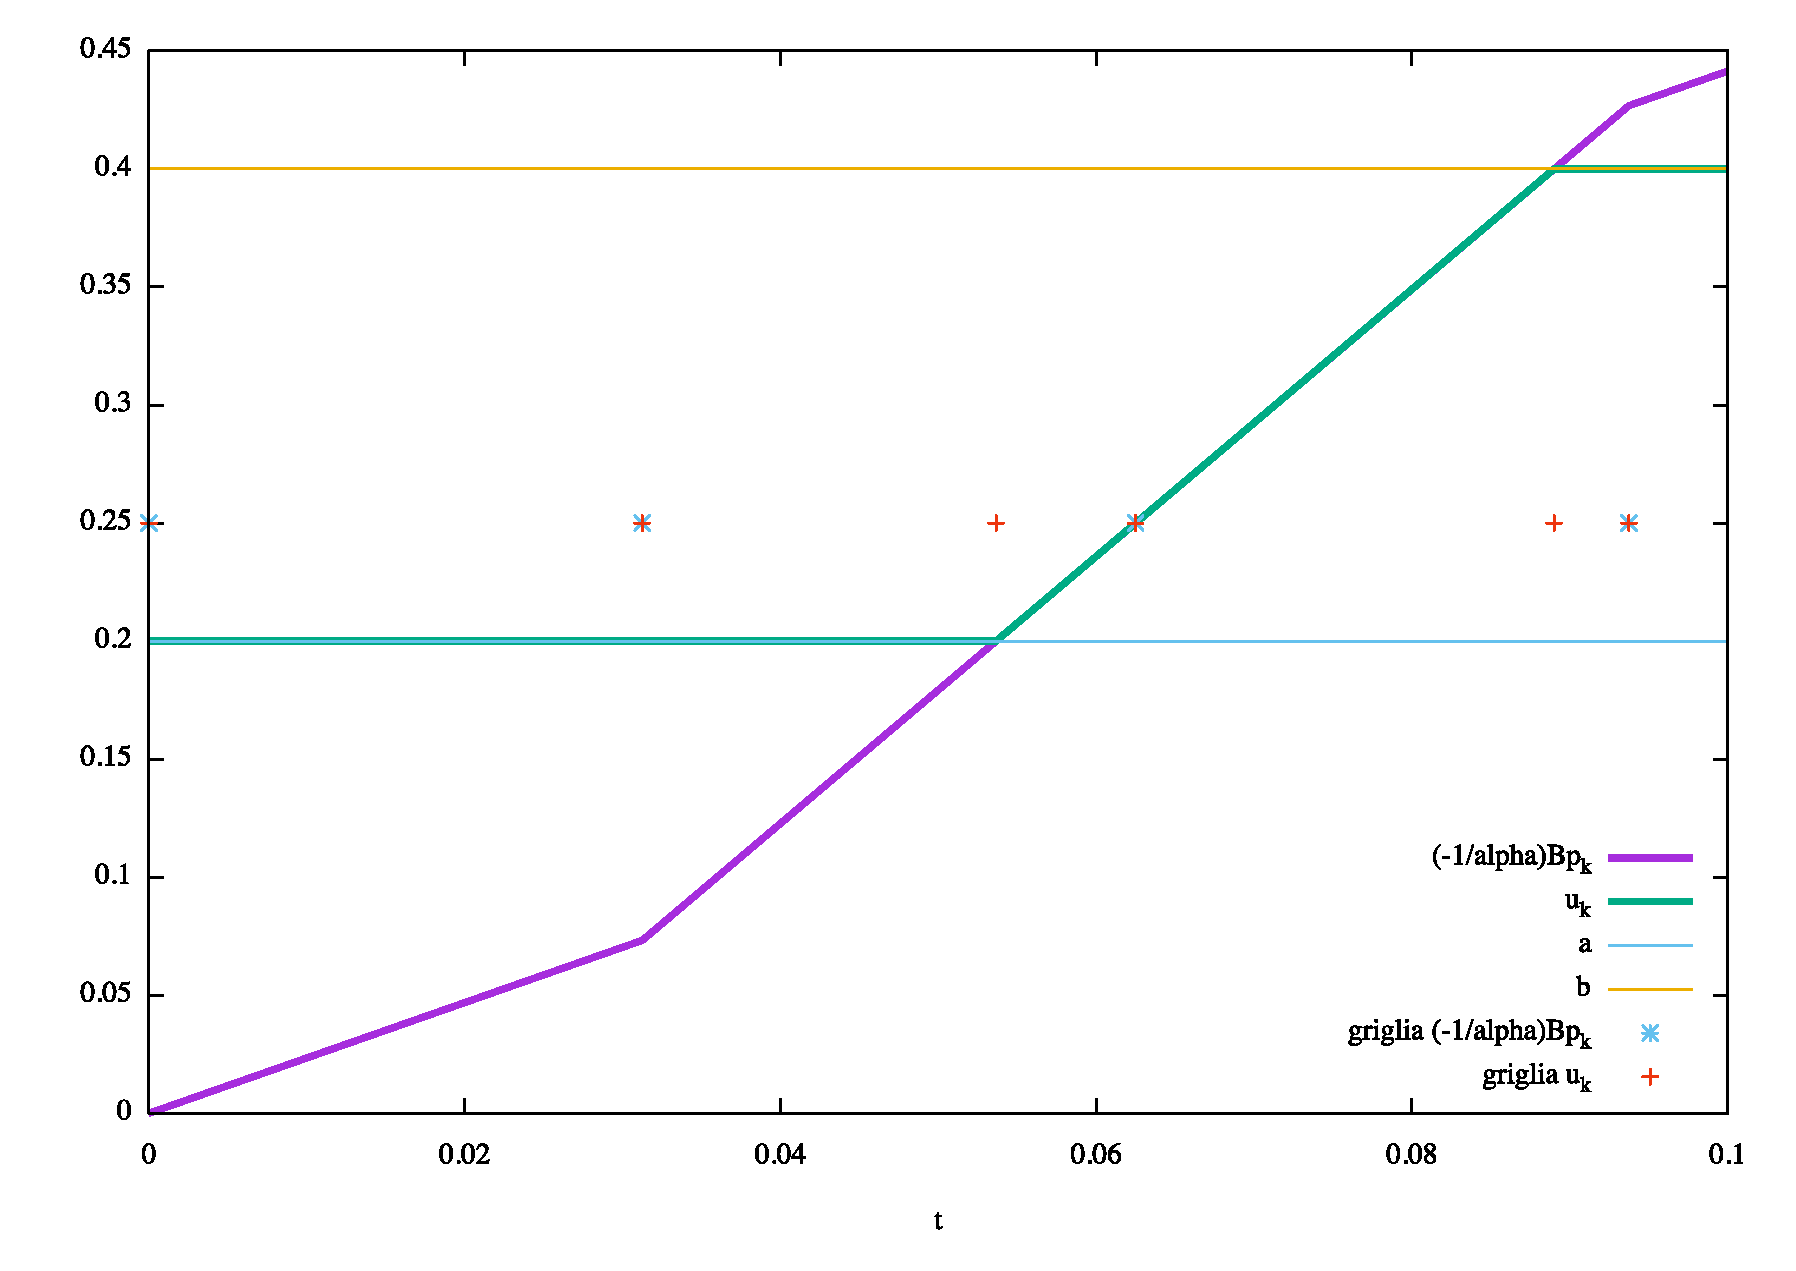
\includegraphics[scale=0.25]{img/cap5/griglie}
\label{fig:griglie}
\end{figure}

l'operazione di proiezione $P_{U_{ab}}$ non garantisce che i nodi della griglia temporale utilizzata corrispondano a i punti di non derivabilità della funzione proiettata

\end{frame}

\begin{frame}
\frametitle{Implementazione: Schema Problema di Stato}
%Lo schema di integrazione temporale per il problema di stato è una variante dello schema di Crank-Nicolson.
Considerato la matrice di Stiffness ed il temine noto al passo k:
\begin{multline*}
A(y_k,y_{test}) = \int_{\Omega} \gamma_1 \bigtriangledown y_k \bigtriangledown y_{test} \, d\Omega 
\end{multline*}
\begin{multline*}
b(y_{test}) = \int_{\Omega} \gamma_2 \bigtriangledown y_{k-1} \bigtriangledown y_{test} \, d\Omega \\+ \int_{\Omega} \gamma_3 (f_{k}+u_k)y_{test} \, d\Omega + \int_{\Omega} \gamma_4 (f_{k-1}+u_{k-1})y_{test} \, d\Omega
\end{multline*}

\begin{table}
\centering
\begin{tabular}{|c|c|c|c|c|}
\hline
\textbf{Schema} & \textbf{$\gamma_1$} &\textbf{$\gamma_2$} & \textbf{$\gamma_3$} &\textbf{$\gamma_4$} \\
\hline
EI & 0.5 & 0 & 0 & 0.5 \\
\hline
CN & 0.5 & 0.5 & 0 & 1 \\
\hline
EA & 0 & 0.5 & 0.5 & 0\\
\hline
\end{tabular}
\end{table}
\end{frame}

\begin{frame}
\frametitle{Implementazione: Forzante del Problema Aggiunto}
Anche per il problema aggiunto è stato utilizzato un metodo di Crank-Nicolson con la matrice di Stiffness ed il termine noto al passo i:
\begin{multline*}
A(p_i,p_{test}) = \int_{\Omega} \frac{1}{2}\bigtriangledown p_i \bigtriangledown p_{test} \, d\Omega 
\end{multline*}
\begin{multline*}
b(p_{test}) = \int_{\Omega} \frac{1}{2} \bigtriangledown p_{i+1} \bigtriangledown p_{test} \, d\Omega \\+ \int_{\Omega} \frac{1}{2} h_i p_{test} \, d\Omega + \int_{\Omega} \frac{1}{2} h_{i+1} p_{test} \, d\Omega
\end{multline*}
dove:
\begin{equation*}
h_i = {y_k}_i - y_d(t_i), \quad
h_{i+1} = {y_k}_i - y_d(t_i+{\Delta}t)
\end{equation*}

\end{frame}

\begin{frame}
\frametitle{Implementazione Semi-Newton}
Per risolvere l'equazione:

\begin{equation*}
\big( I + \frac{1}{\alpha}S_h\mathbbm{1}_{S^*_hw}S^*_h\big)\delta w=-(w+y_d)+S_hP{U_{ad}}\big( -\frac{1}{\alpha}S^*_hw\big).
\end{equation*}

è stato implementato il metodo del gradiente coniugato.
\\
La funzione \texttt{adjCG(real[int,int] \&xx)} implementa l’operatore ${S_h}^*$; 
%Il procedimento utilizzato rispecchia quello precedentemente implementato per il metodo di punto fisso.

\end{frame}

\begin{frame}
\frametitle{Funzioni per l'operatore di stato}
Per la soluzione dell'operatore di stato son state implementate due diverse funzioni.
\texttt{stateCG(real[int] \&xx)} risolve l'operatore $S_h$ applicato a $P_{U_{ad}}(xx)$ con termine noto al passo k:
\begin{multline*}
b(y_{test}) = \int_{\Omega} \gamma_2 \bigtriangledown y_{k-1} \bigtriangledown y_{test} \, d\Omega \\+ \int_{\Omega} \gamma_3 (f_{k}+P_{U_{ad}}(xx_k))y_{test} \, d\Omega + \int_{\Omega} \gamma_4 (f_{k-1}+P_{U_{ad}}(xx_{k-1}))y_{test} \, d\Omega
\end{multline*}

\texttt{mat1(real[int] \&xx, real[int] \&ww)} risolve l'operatore $S_h\mathbbm{1}_{S^*_hw}$ considerato con termine noto al passo k:
\begin{multline*}
b(y_{test}) = \int_{\Omega} \gamma_2 \bigtriangledown y_{k-1} \bigtriangledown y_{test} \, d\Omega \\+ \int_{\Omega} \gamma_3 \chi_{U_{ad}}xx_k y_{test} \, d\Omega + \int_{\Omega} \gamma_4 \chi_{U_{ad}}xx_{k-1} y_{test} \, d\Omega
\end{multline*}

\end{frame}

\section{Risultati}


\begin{frame}
\frametitle{Test Case 01 ed 02: dati del problema}

Per entrambi i test case considera $\Omega = (0,1)^2$.
Viene utilizzata una mesh spaziale uniforme con 22801 nodi.

\begin{table}
\centering
\begin{tabular}{|c|c|c|}
\hline
\textbf{Parametro} & \textbf{TestCase01} & \textbf{TestCase02} \\
\hline
I & (0,0.1) & (0,0.5) \\
\hline
$U_{ad}$ & a=-25 ed b =-1 & a=0.2 ed b=0.4 \\
\hline
$\alpha$ & $\pi^{-4}$ & 1 \\
\hline
\end{tabular}
\end{table}

\end{frame}

\subsection{Test Case 01}
\begin{frame}
\frametitle{Test Case 01 Punto fisso $\overline{u}$ e $u_k$}

\begin{figure}
\centering
\subfigure[{l = 1}]%
{\includegraphics[width=0.25\linewidth]{img/cap6/Imm_PF_01/ControlSol_N150_l1}}\qquad
\subfigure[\protect\url{l = 2}]%
{\includegraphics[width=0.25\linewidth]{img/cap6/Imm_PF_01/ControlSol_N150_l2}}\qquad
\subfigure[\protect\url{l = 3}]%
{\includegraphics[width=0.25\linewidth]{img/cap6/Imm_PF_01/ControlSol_N150_l3}}\qquad
\subfigure[\protect\url{l = 4}]%
{\includegraphics[width=0.25\linewidth]{img/cap6/Imm_PF_01/ControlSol_N150_l4}}\qquad
\subfigure[\protect\url{l = 5}]%
{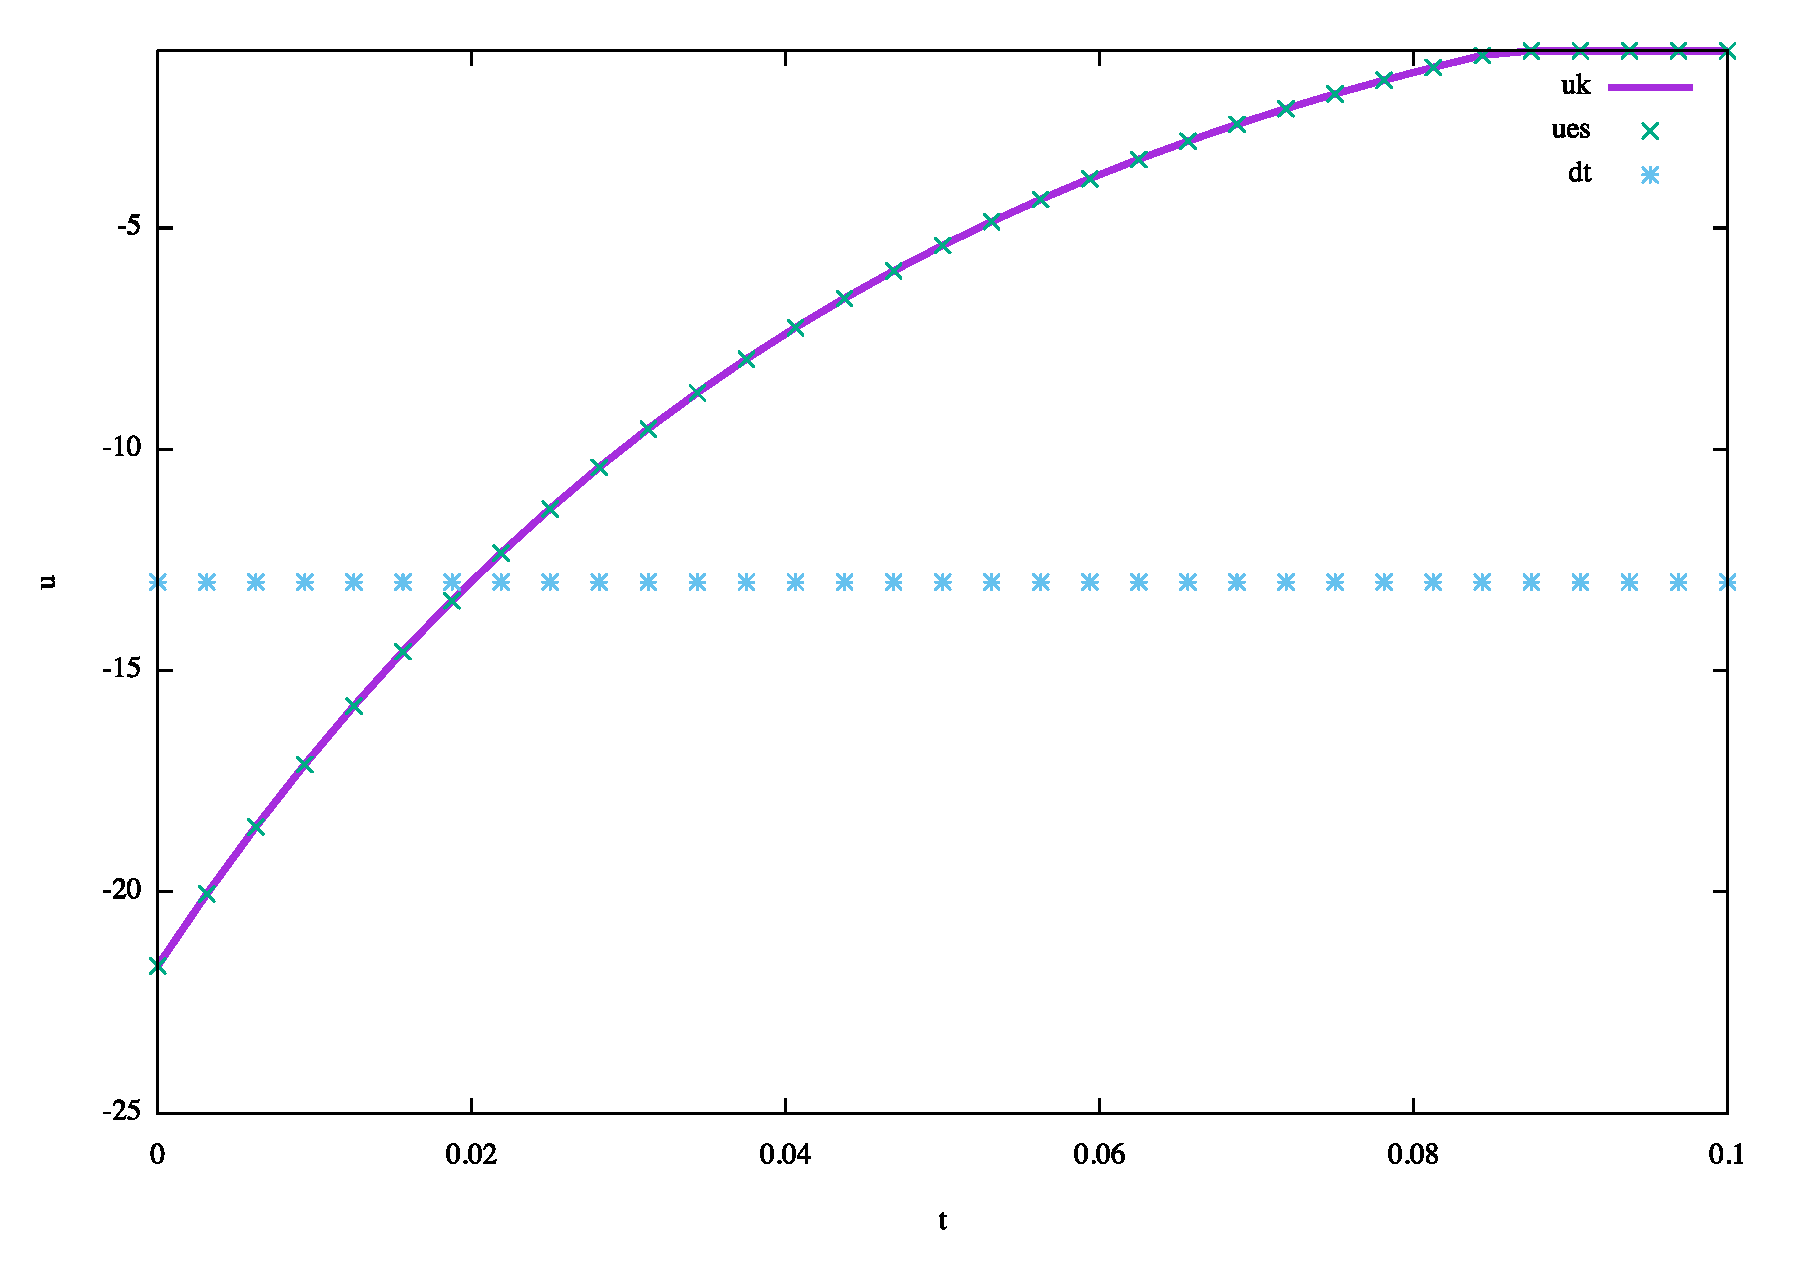
\includegraphics[width=0.25\linewidth]{img/cap6/Imm_PF_01/ControlSol_N150_l5}}\qquad
\subfigure[\protect\url{l = 6}]%
{\includegraphics[width=0.25\linewidth]{img/cap6/Imm_PF_01/ControlSol_N150_l6}}
\label{fig:501}
\end{figure}

\end{frame}

\begin{frame}
\frametitle{Test Case 01 Punto fisso}
\begin{table}
\caption{Punto fisso per Test case 01: errori e EOC }
\label{puntofissoI}
\centering

\begin{tabular}{cllll}
\toprule
{l}           &  {$ \norma{\bar{u}-u_{kh}}_{L^2(L^2)} $} &  {$ \norma{\bar{y}-y_{kh}}_{L^2(L^2)} $} &  {$ EOC_u $} &  {$ EOC_y $} \\
\midrule
1            &  0.31667 &  0.981285 &  {$-$} &  {$-$} \\
2            &  0.0835064 &  0.496296 &  2.60937 &  1.33449 \\
3            &  0.0209608 &  0.248822 &  2.35165 &  1.17464 \\
4            &  0.00500916 &  0.124494 &  2.25065 &  1.08882 \\
5            &  0.00109219  &  0.0622586 &  2.29624 &  1.04473 \\
6            &  0.000497644 &  0.0311327 &  1.15957 &  1.02236 \\
\bottomrule
\end{tabular}              
\end{table}

\end{frame}

\begin{frame}
\frametitle{Test Case 01 Punto fisso}

\begin{table}
\caption{Punto fisso per Test case 01: errori e EOC }
\label{puntofissoIbis}
\centering

\begin{tabular}{cllll}
\toprule
{l}           &  {$ \norma{\bar{y}-\pi_{P^*_k}y_{kh}}_{L^2(L^2)} $} &  {$ \norma{\bar{p}-p_{kh}}_{L^2(L^2)} $} &  {$ EOC_{\pi y} $} &  {$ EOC_p $} \\
\midrule
1            &  0.520894 &  0.00660747 &  {$-$} &  {$-$} \\
2            &  0.15134 &  0.00173155 &  2.41965 &  2.6216 \\
3            &  0.0393476 &  0.00043334 &  2.29181 &  2.35673 \\
4            &  0.00970087 &  0.000103613 &  2.20164 &  2.24982 \\
5            &  0.00221619 &  0.000022824 &  2.2259 &  2.28078 \\
6            &  0.000432024 &  0.000010724 &  2.41203 &  1.11429 \\
\bottomrule
\end{tabular}              
\end{table}

\end{frame}

\begin{frame}
\frametitle{Test Case 01 Semi-Newton}
\begin{figure}
\centering%
\subfigure[{l = 1}]%
{\includegraphics[width=0.25\linewidth]{img/cap6/Imm_CG_01/ControlSol_N150_l1}}\qquad
\subfigure[\protect\url{l = 2}]%
{\includegraphics[width=0.25\linewidth]{img/cap6/Imm_CG_01/ControlSol_N150_l2}}\qquad
\subfigure[\protect\url{l = 3}]%
{\includegraphics[width=0.25\linewidth]{img/cap6/Imm_CG_01/ControlSol_N150_l3}}\qquad
\subfigure[\protect\url{l = 4}]%
{\includegraphics[width=0.25\linewidth]{img/cap6/Imm_CG_01/ControlSol_N150_l4}}\qquad
\subfigure[\protect\url{l = 5}]%
{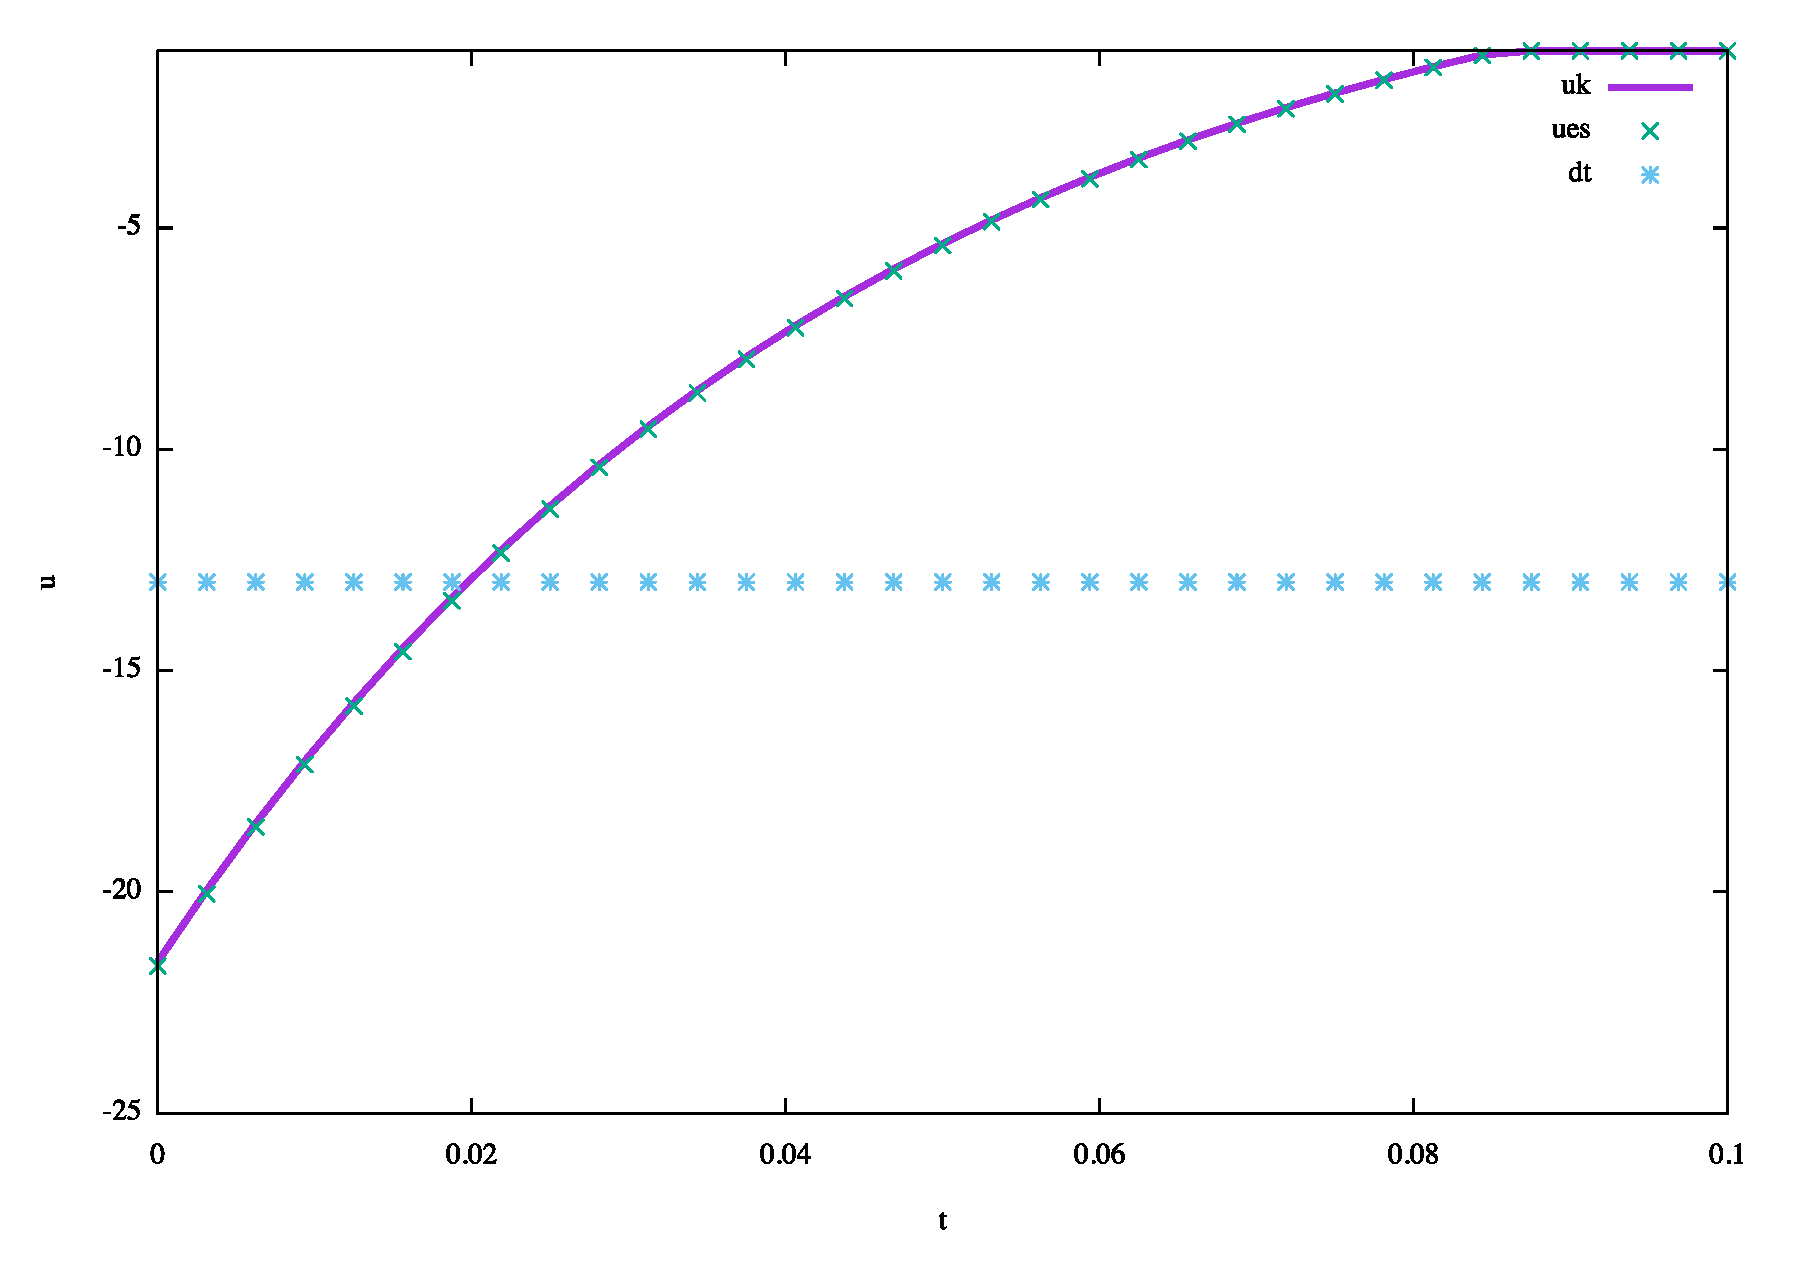
\includegraphics[width=0.25\linewidth]{img/cap6/Imm_CG_01/ControlSol_N150_l5}}\qquad
\subfigure[\protect\url{l = 6}]%
{\includegraphics[width=0.25\linewidth]{img/cap6/Imm_CG_01/ControlSol_N150_l6}}
%\caption{Test Case 01 $\overline{u}$ e $u_k$: risultati dell'algortimo semi Newton}
\label{fig:502}
\end{figure}

\end{frame}

\begin{frame}
\frametitle{Test Case 01 Semi-Newton}

\begin{table}
\caption{Newton per Test case 01: errori e EOC }
\label{newtonI}
\centering

\begin{tabular}{cllll}
\toprule
{l}           &  {$ \norma{\bar{u}-u_{kh}}_{L^2(L^2)} $} &  {$ \norma{\bar{y}-y_{kh}}_{L^2(L^2)} $} &  {$ EOC_u $} &  {$ EOC_y $} \\
\midrule
1            &  0.316669 &  0.981285 &  {$-$} &  {$-$} \\
2            &  0.0835064 &  0.496296 &  2.60937 &  1.33449 \\
3            &  0.0209612 &  0.248822 &  2.35161 &  1.17464 \\
4            &  0.00500971 &  0.124494  &  2.25051 &  1.08882 \\
5            &  0.00109312 &  0.0622586 &  2.29512 &  1.04473 \\
6            &  0.000497833 &  0.0311327 &  1.16028 &  1.02236 \\
\bottomrule
\end{tabular}              
\end{table}

\end{frame}

\begin{frame}
\frametitle{Test Case 01 Semi-Newton}
\begin{table}
\caption{Newton per Test case 01: errori e EOC }
\label{newtonIbis}
\centering

\begin{tabular}{cllll}
\toprule
{l}           &  {$ \norma{\bar{y}-\pi_{P^*_k}y_{kh}}_{L^2(L^2)} $} & {$ \norma{\bar{p}-p_{kh}}_{L^2(L^2)} $} &  {$ EOC_{\pi y} $}  &  {$ EOC_p $} \\
\midrule
1            &  0.520894 &  0.00660747 &  {$-$} &  {$-$} \\
2            &  0.15134 &  0.00173155 &  2.41965 &  2.6216 \\
3            &  0.0393476 &  0.00043334 &  2.29181 &  2.35672 \\
4            &  0.00970089 &  0.000103614 &  2.20164 &  2.24981 \\
5            &  0.00221621 &  0.0000228246 &  2.22589 &  2.28078 \\
6            &  0.000432023 &  0.0000107235 &  2.41204 &  1.11436 \\
\bottomrule
\end{tabular}              
\end{table}

\end{frame}

\subsection{Test Case 02}
\begin{frame}
\frametitle{Test Case 02 Punto fisso $\overline{u}$ e $u_k$}
\begin{figure}
\centering%
\subfigure[{l = 1}]%
{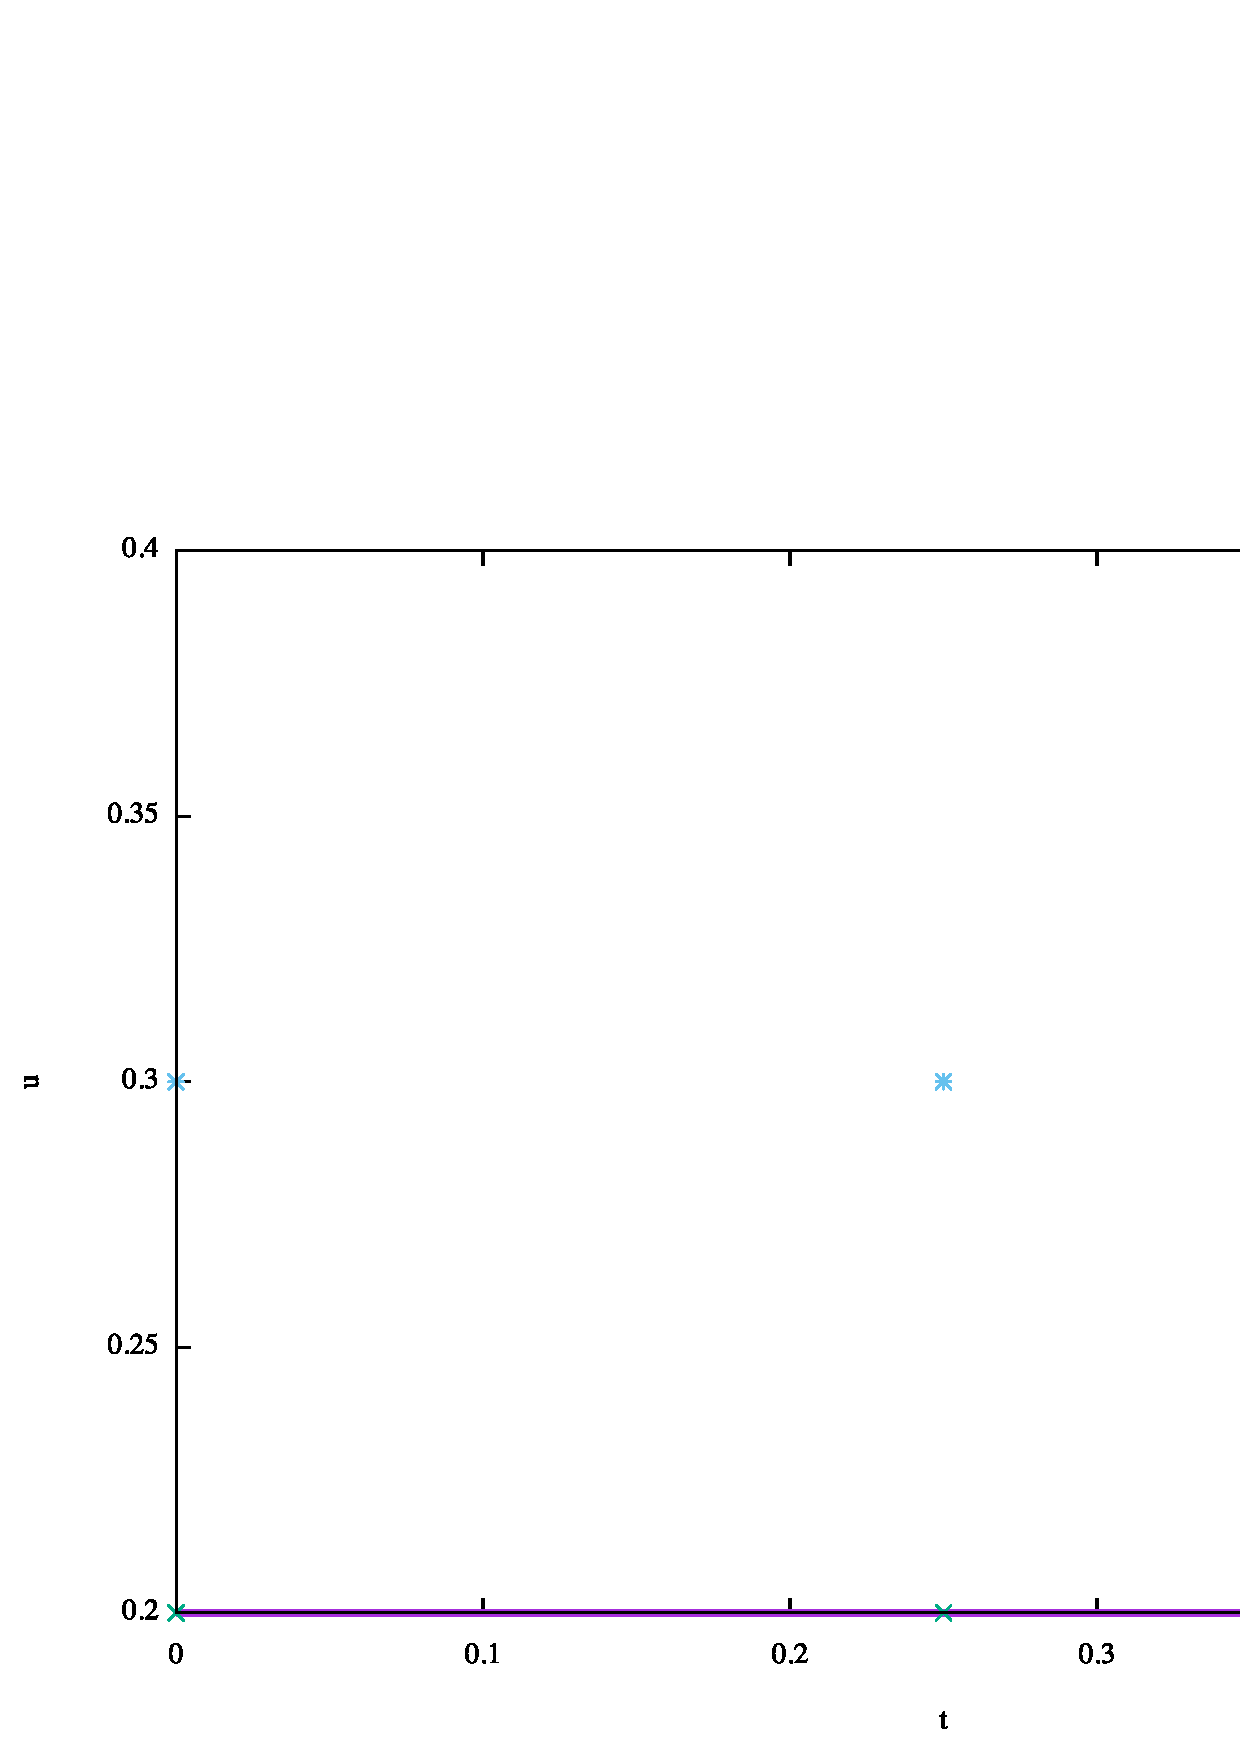
\includegraphics[width=0.2\linewidth]{img/cap6/Imm_PF_02/ControlSol_N150_l1}}\qquad
\subfigure[\protect\url{l = 2}]%
{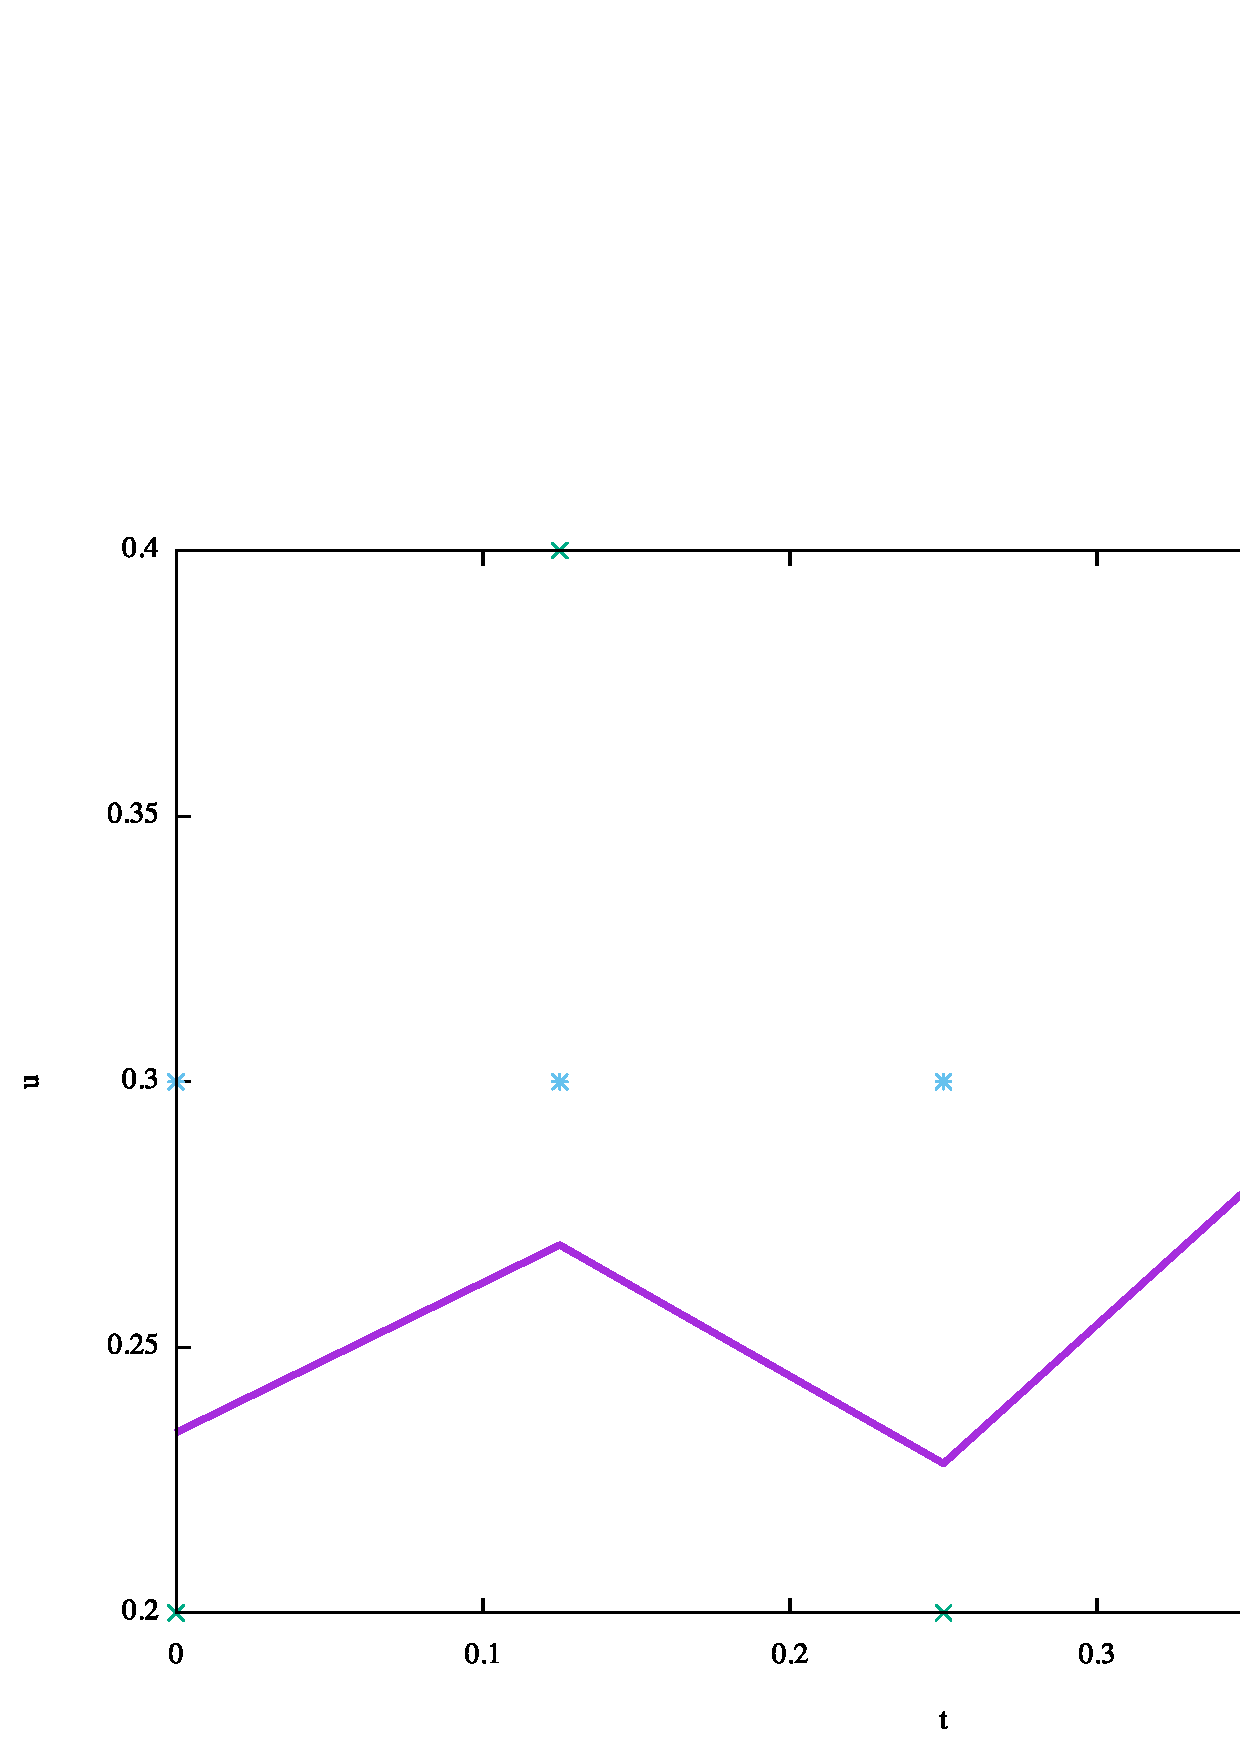
\includegraphics[width=0.2\linewidth]{img/cap6/Imm_PF_02/ControlSol_N150_l2}}\qquad
\subfigure[\protect\url{l = 3}]%
{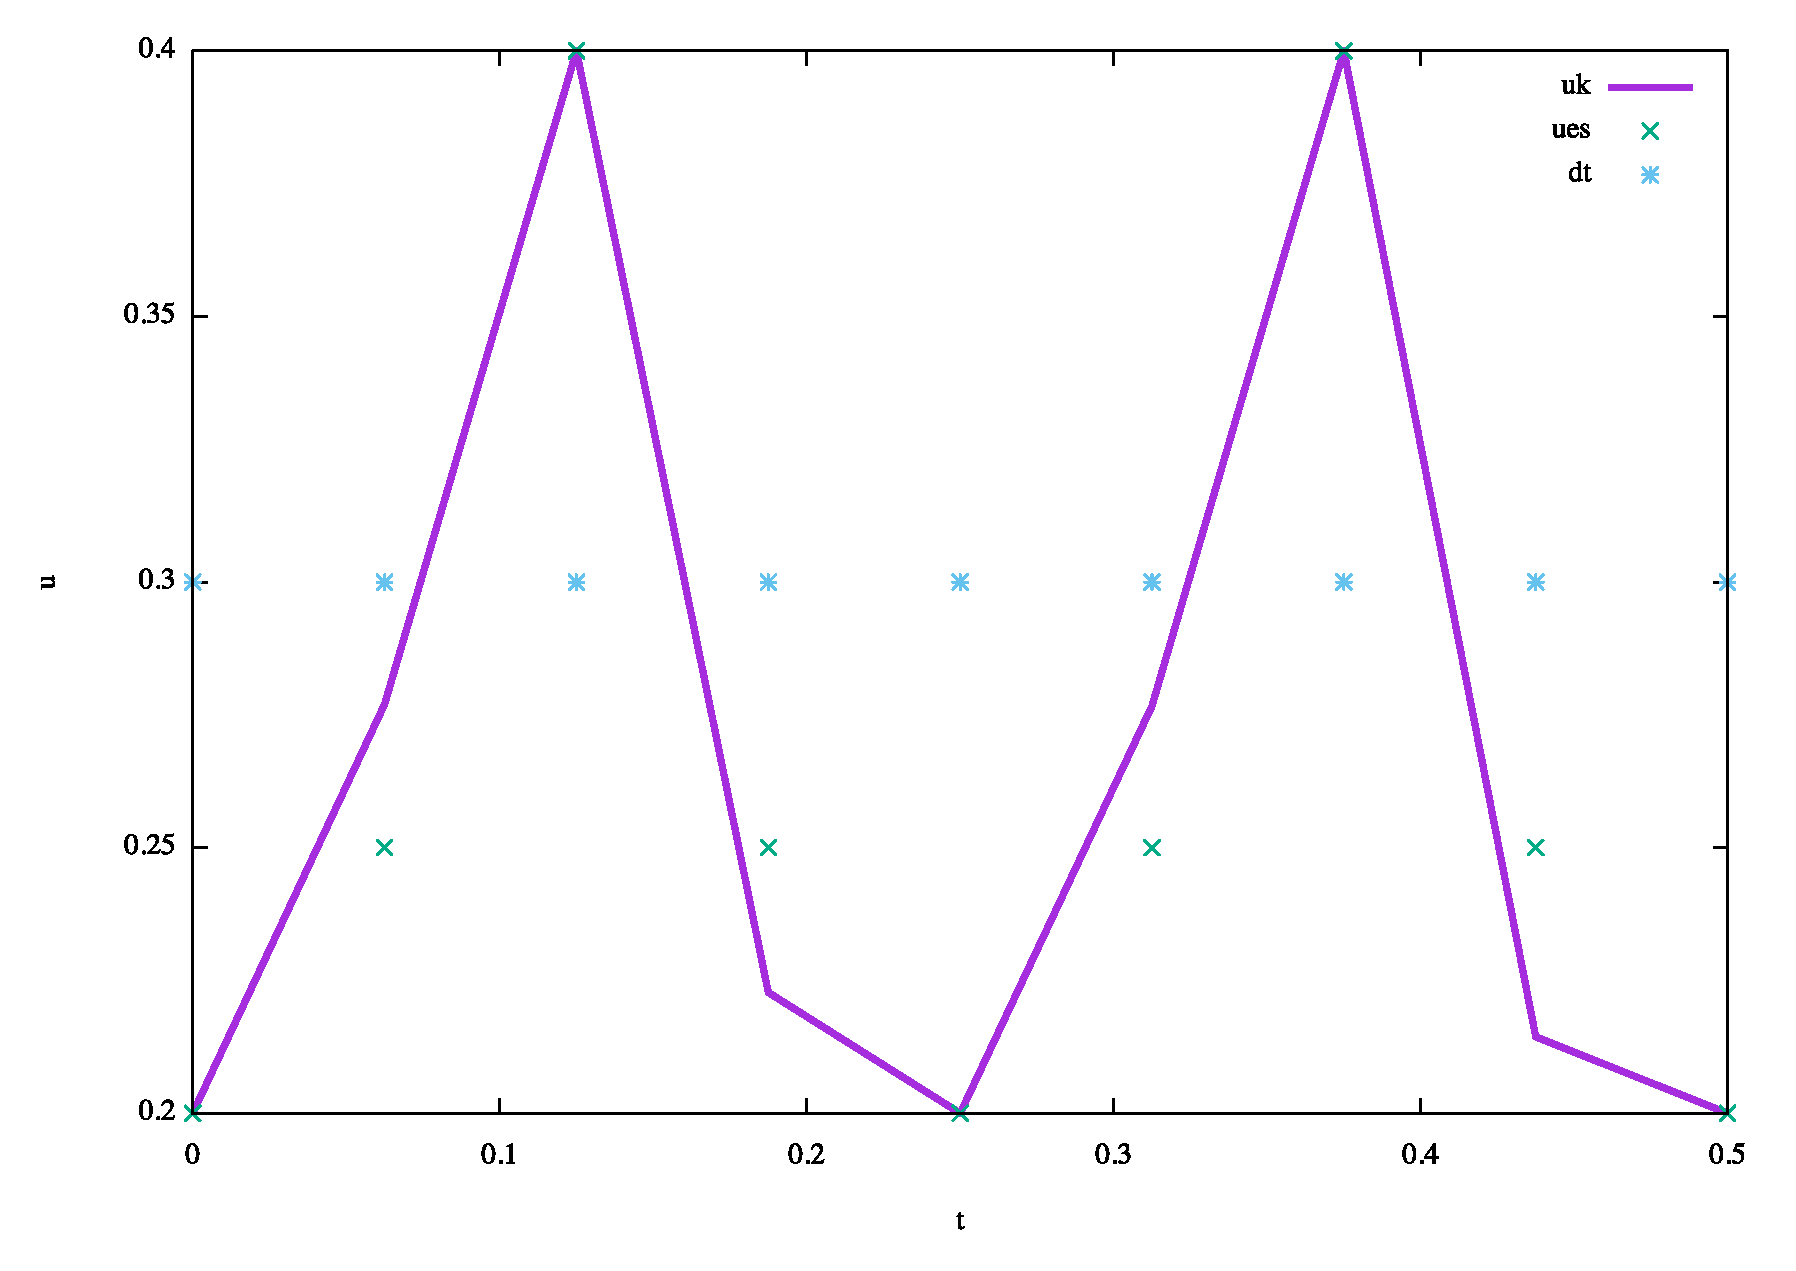
\includegraphics[width=0.2\linewidth]{img/cap6/Imm_PF_02/ControlSol_N150_l3}}\qquad
\subfigure[\protect\url{l = 4}]%
{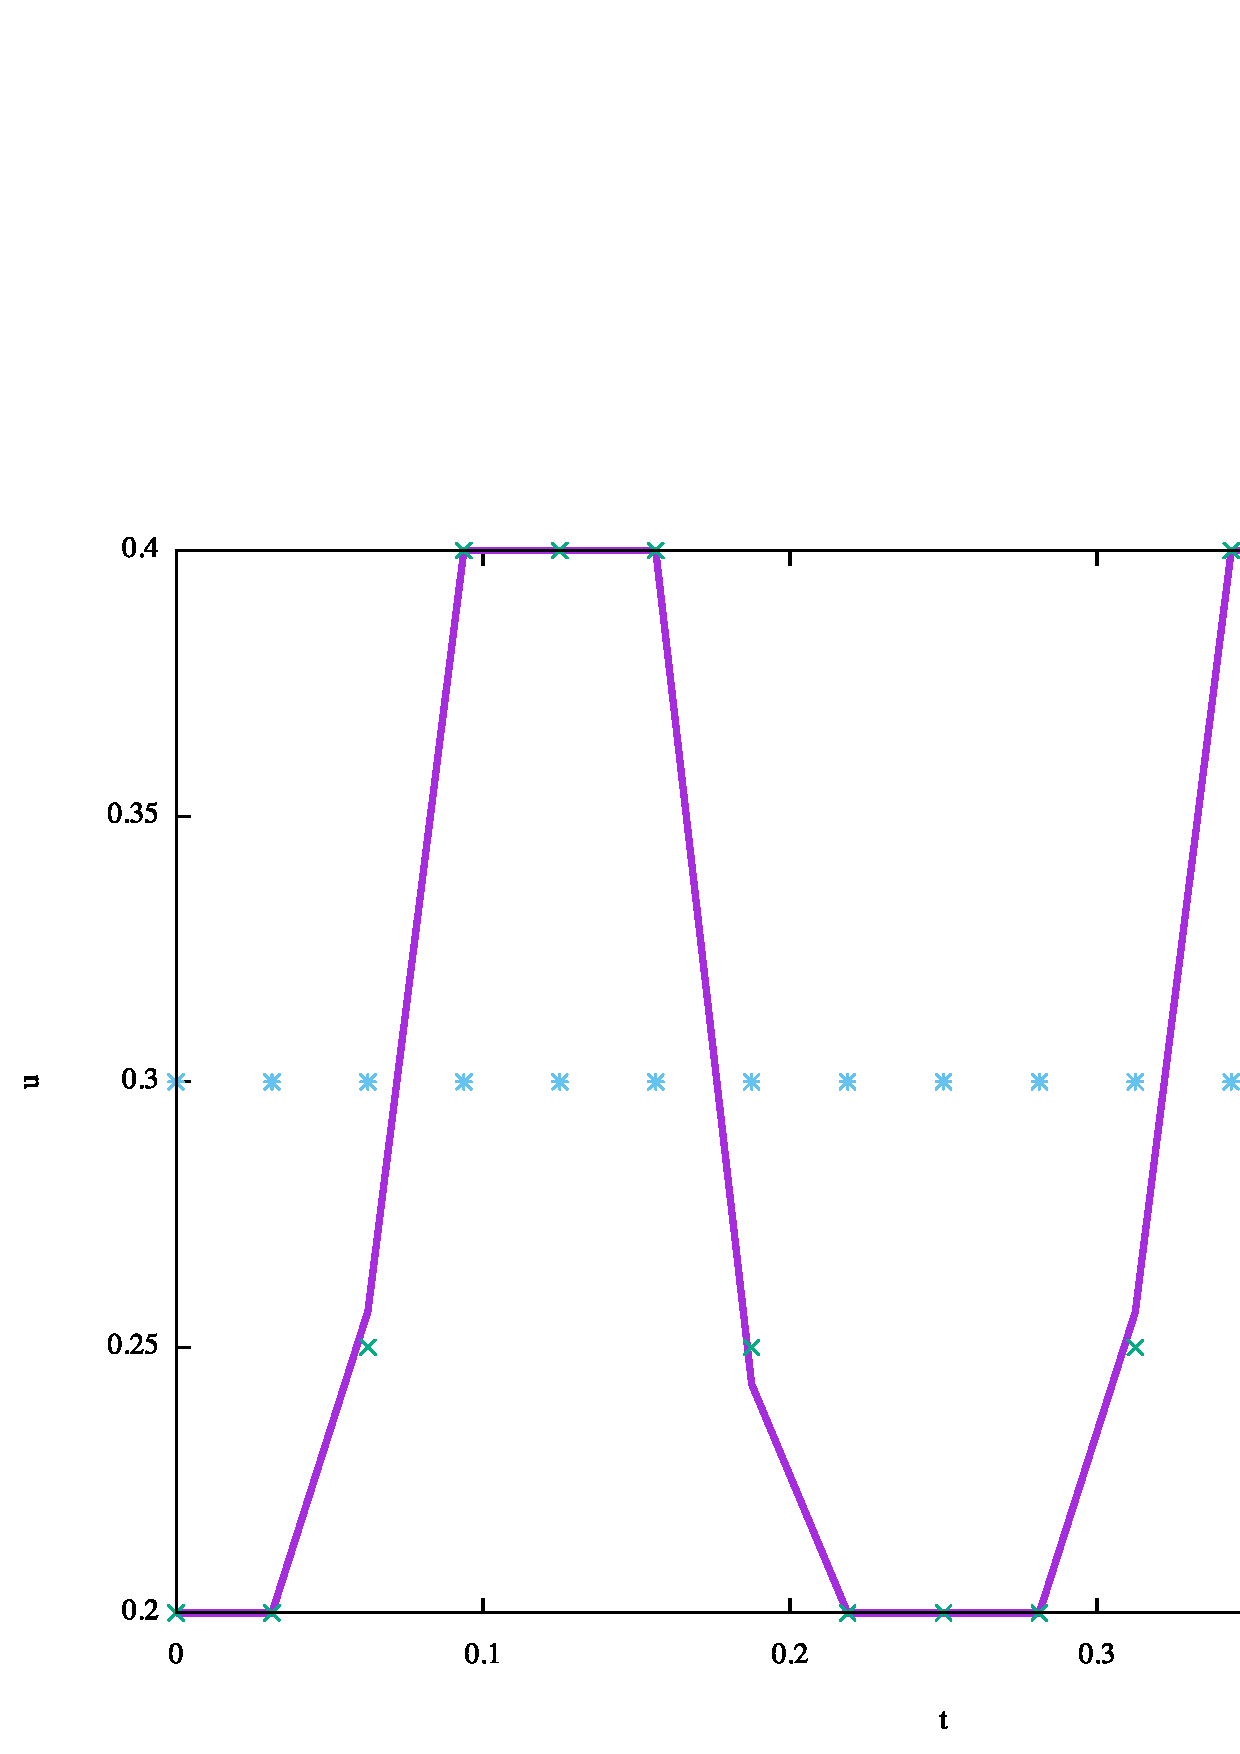
\includegraphics[width=0.2\linewidth]{img/cap6/Imm_PF_02/ControlSol_N150_l4}}\qquad
\subfigure[\protect\url{l = 5}]%
{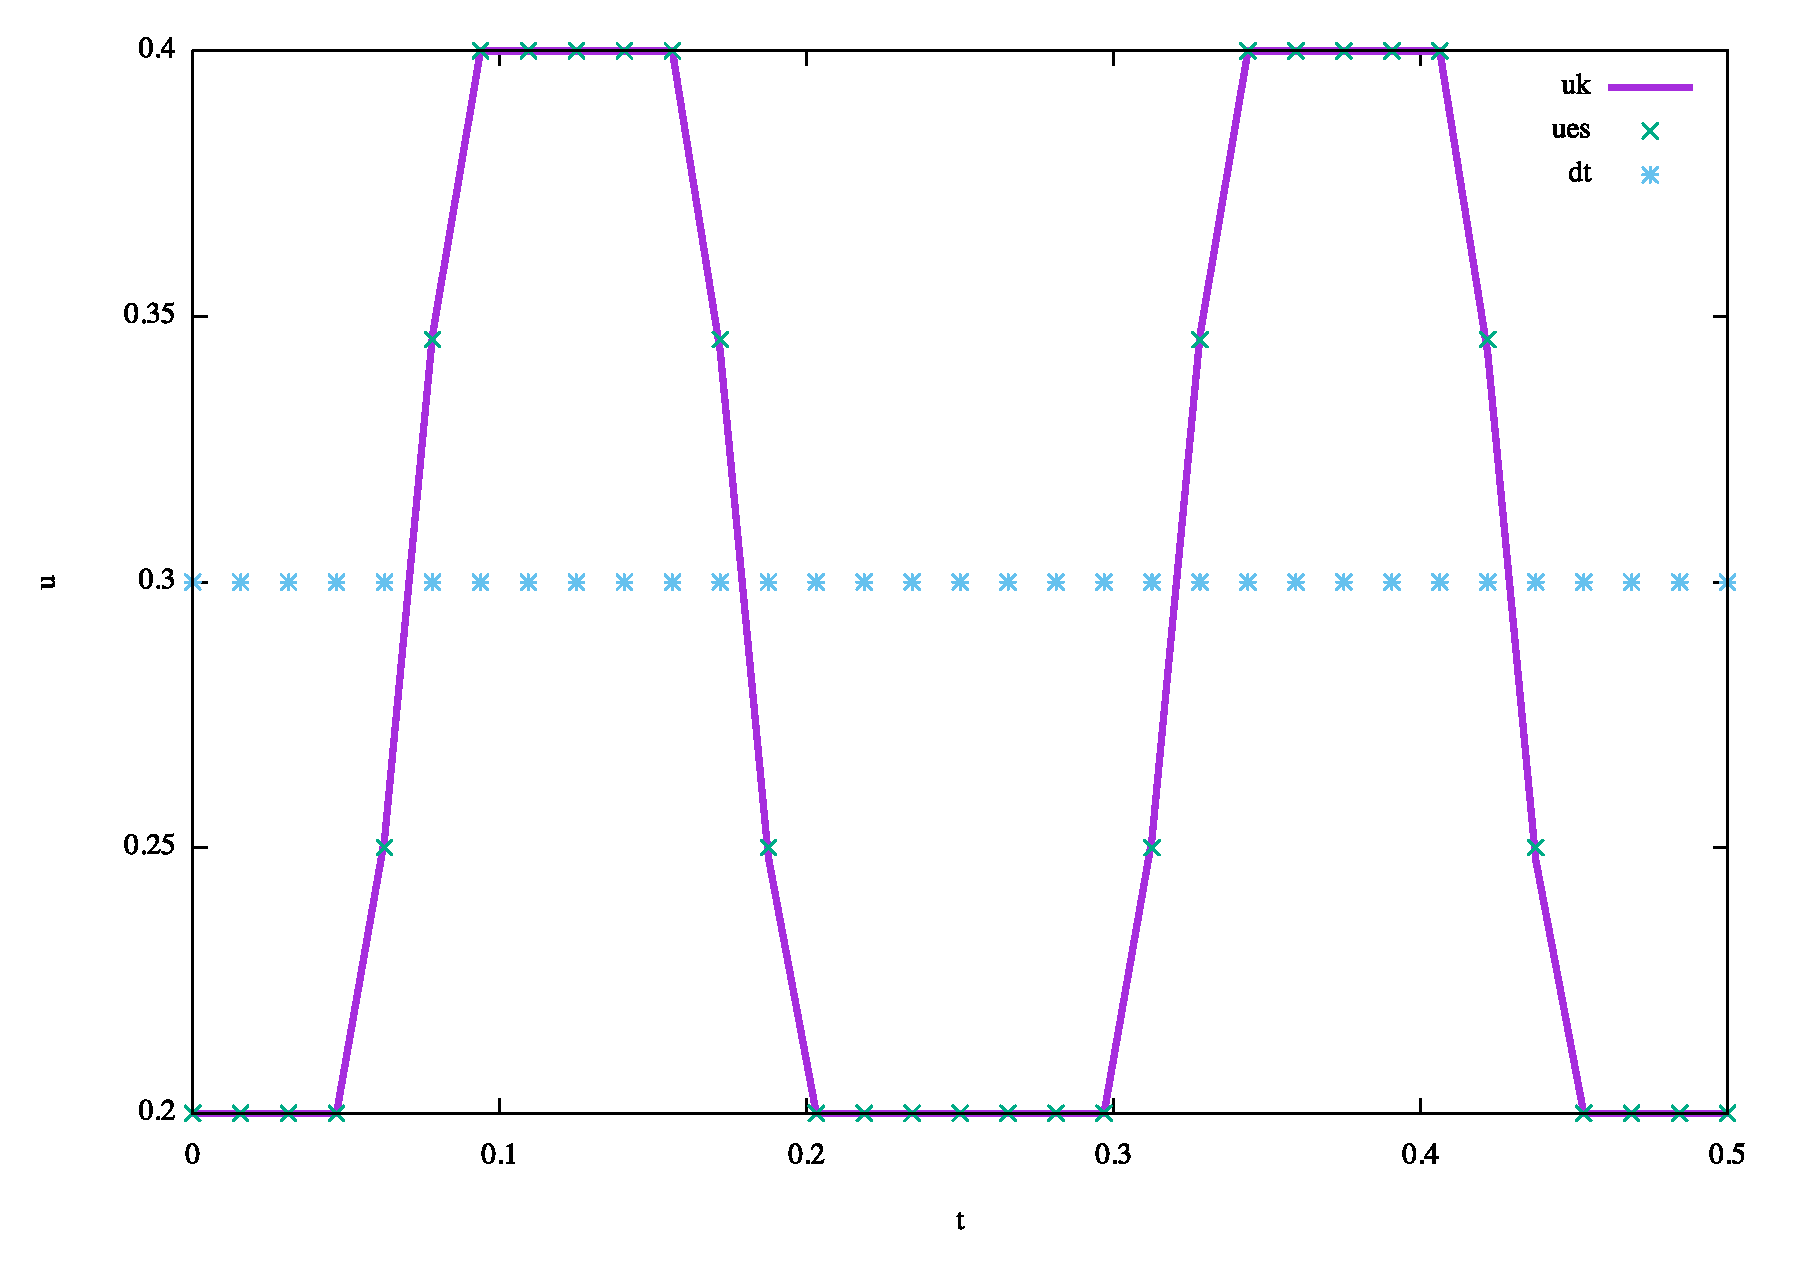
\includegraphics[width=0.2\linewidth]{img/cap6/Imm_PF_02/ControlSol_N150_l5}}\qquad
\subfigure[\protect\url{l = 6}]%
{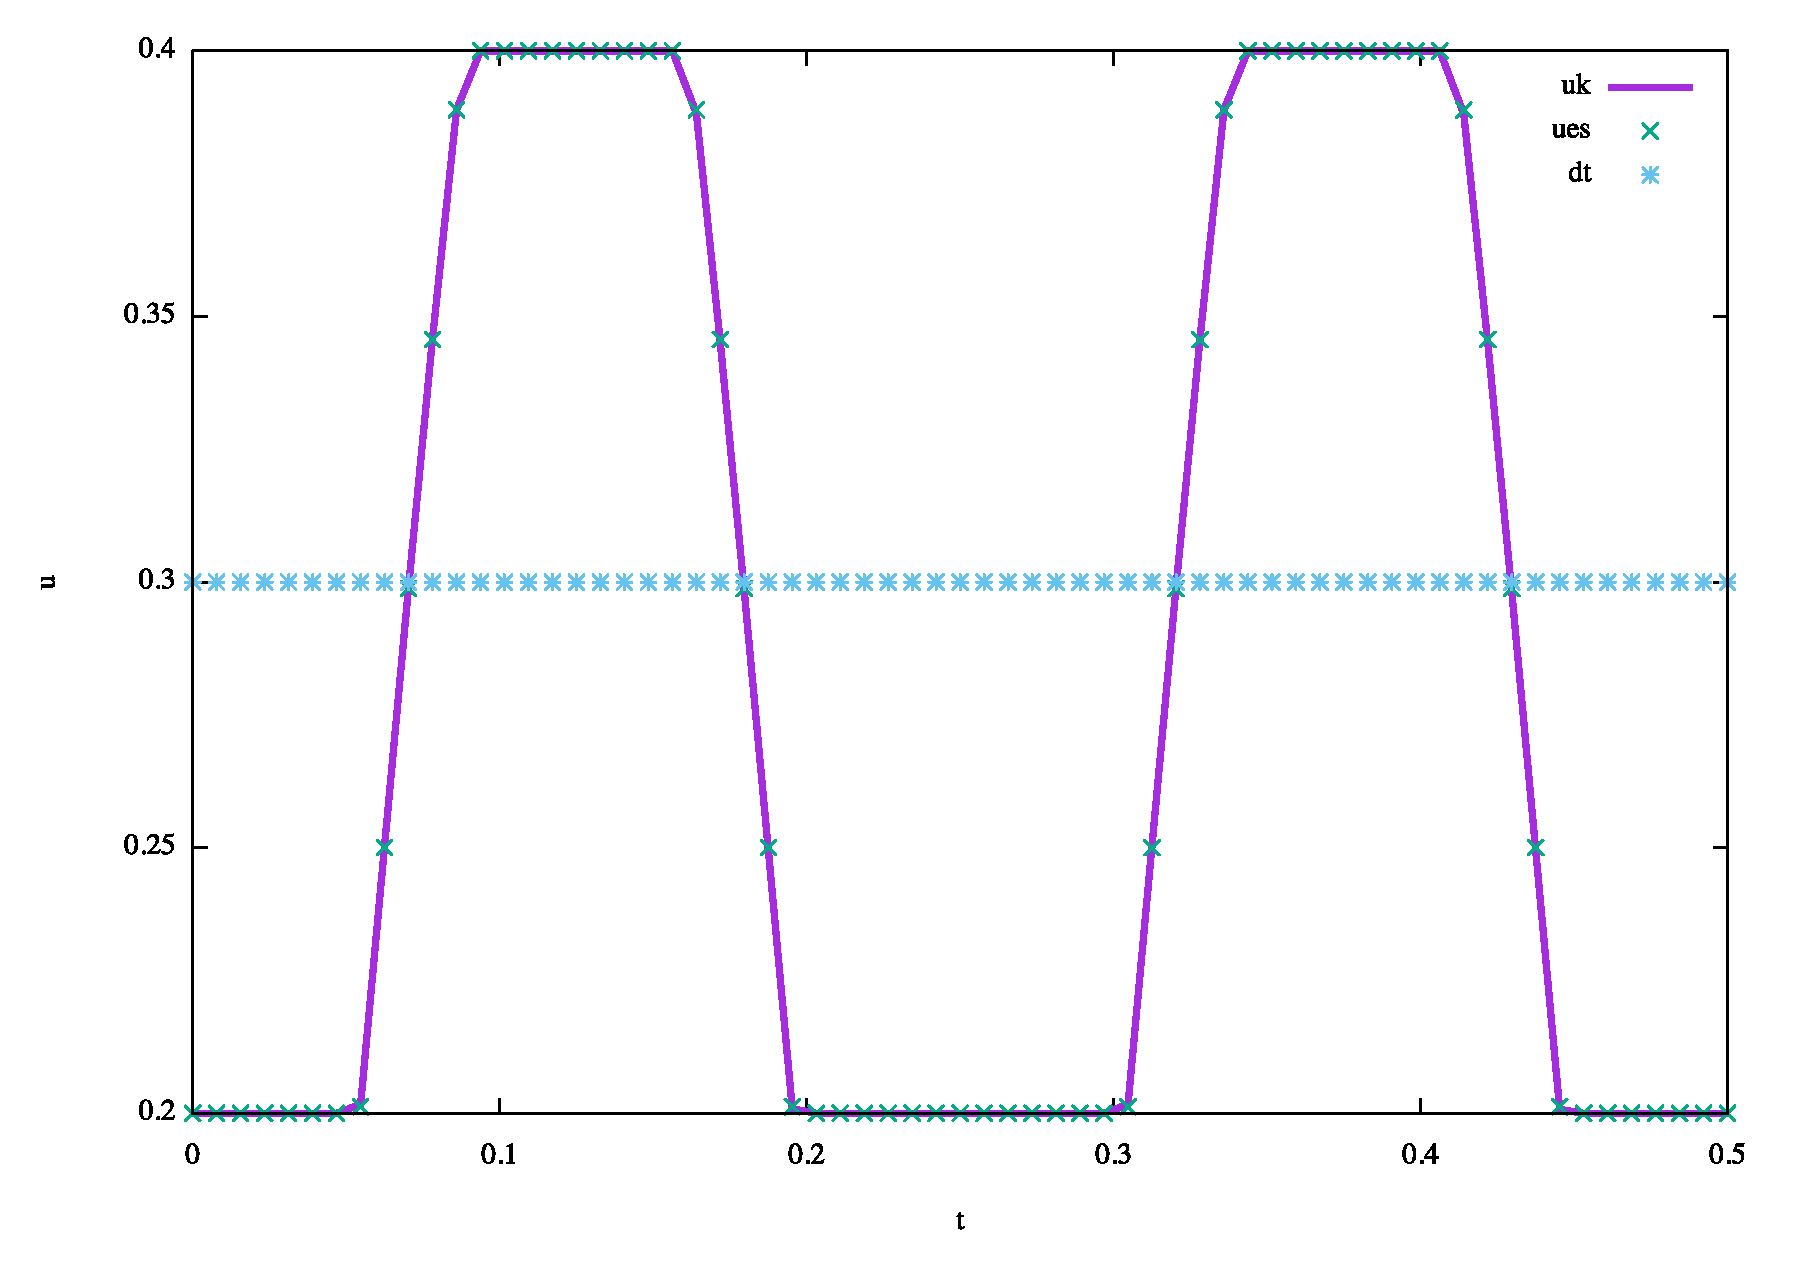
\includegraphics[width=0.2\linewidth]{img/cap6/Imm_PF_02/ControlSol_N150_l6}}\qquad
\subfigure[\protect\url{l = 7}]%
{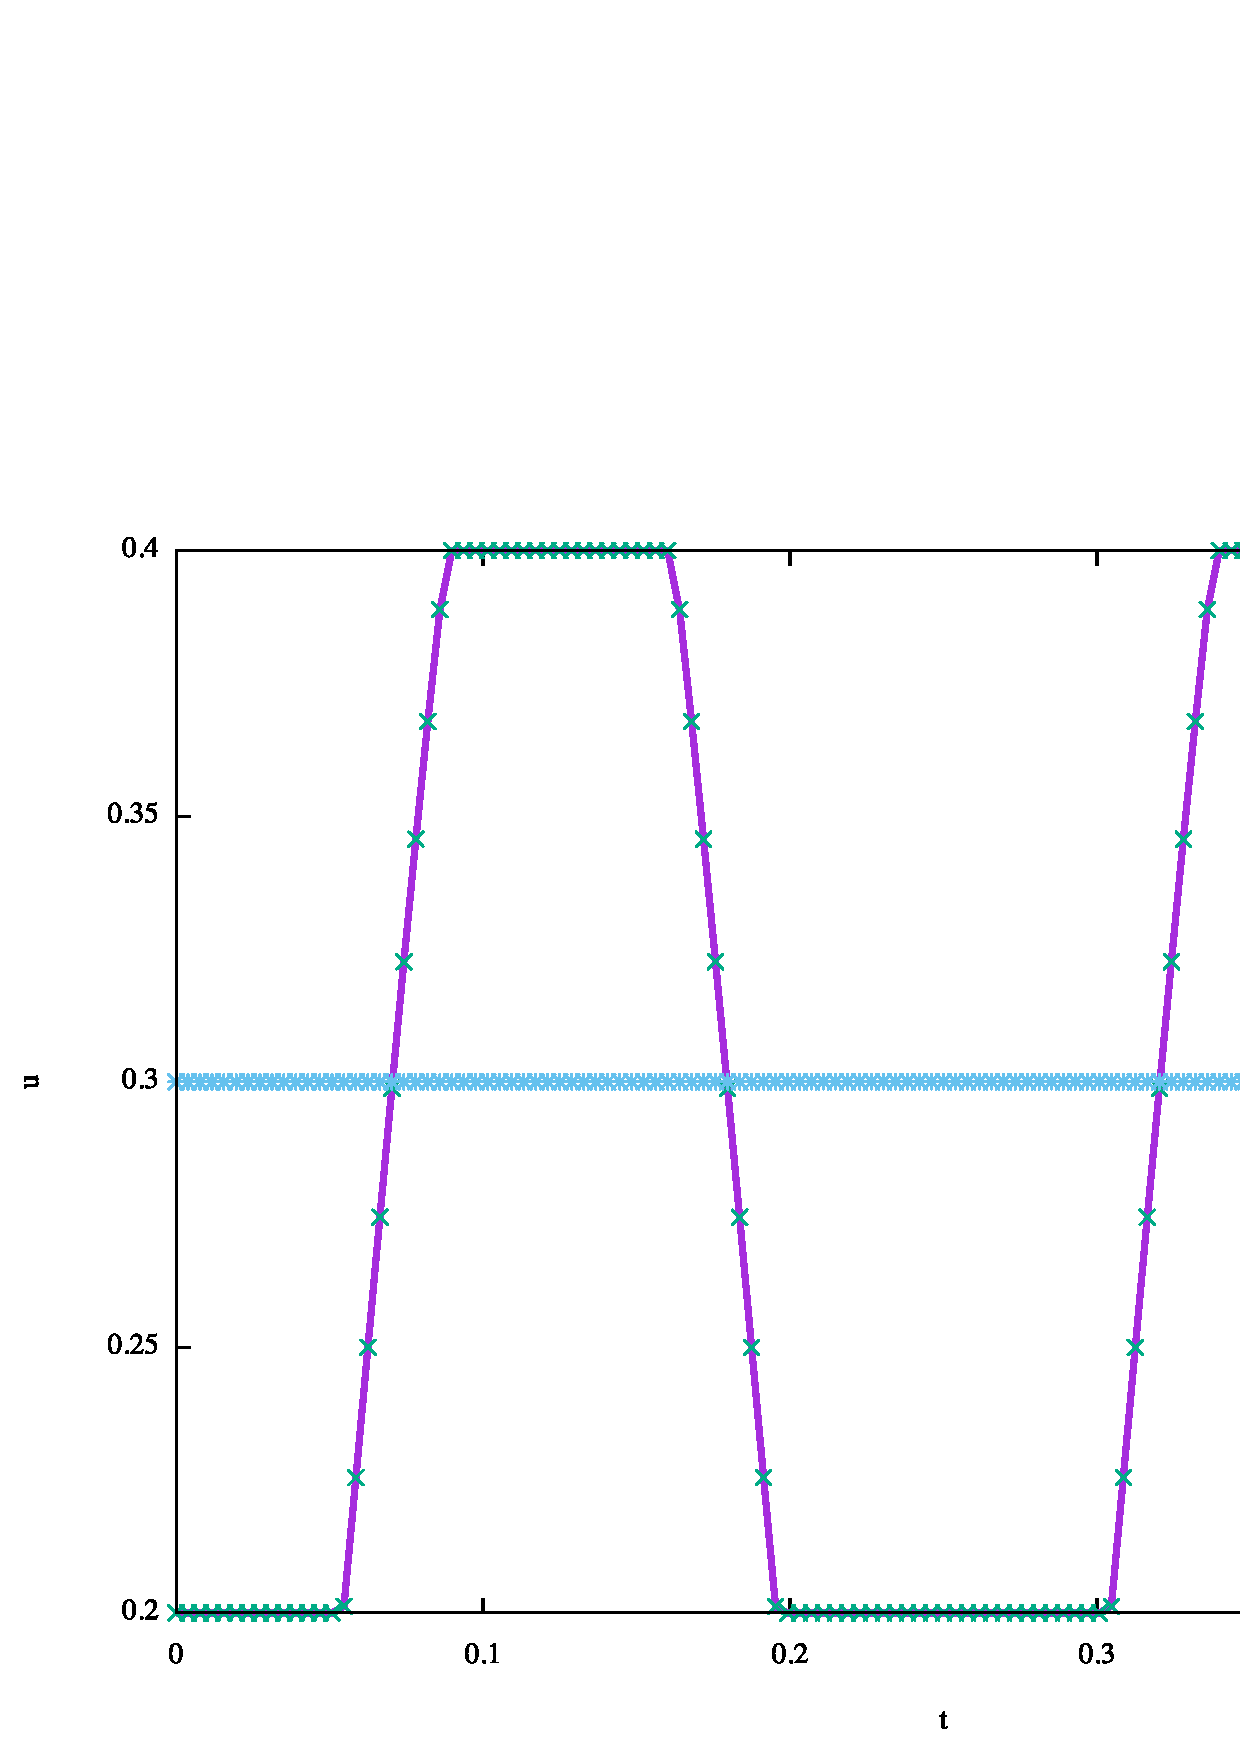
\includegraphics[width=0.2\linewidth]{img/cap6/Imm_PF_02/ControlSol_N150_l7}}\qquad
\subfigure[\protect\url{l = 8}]%
{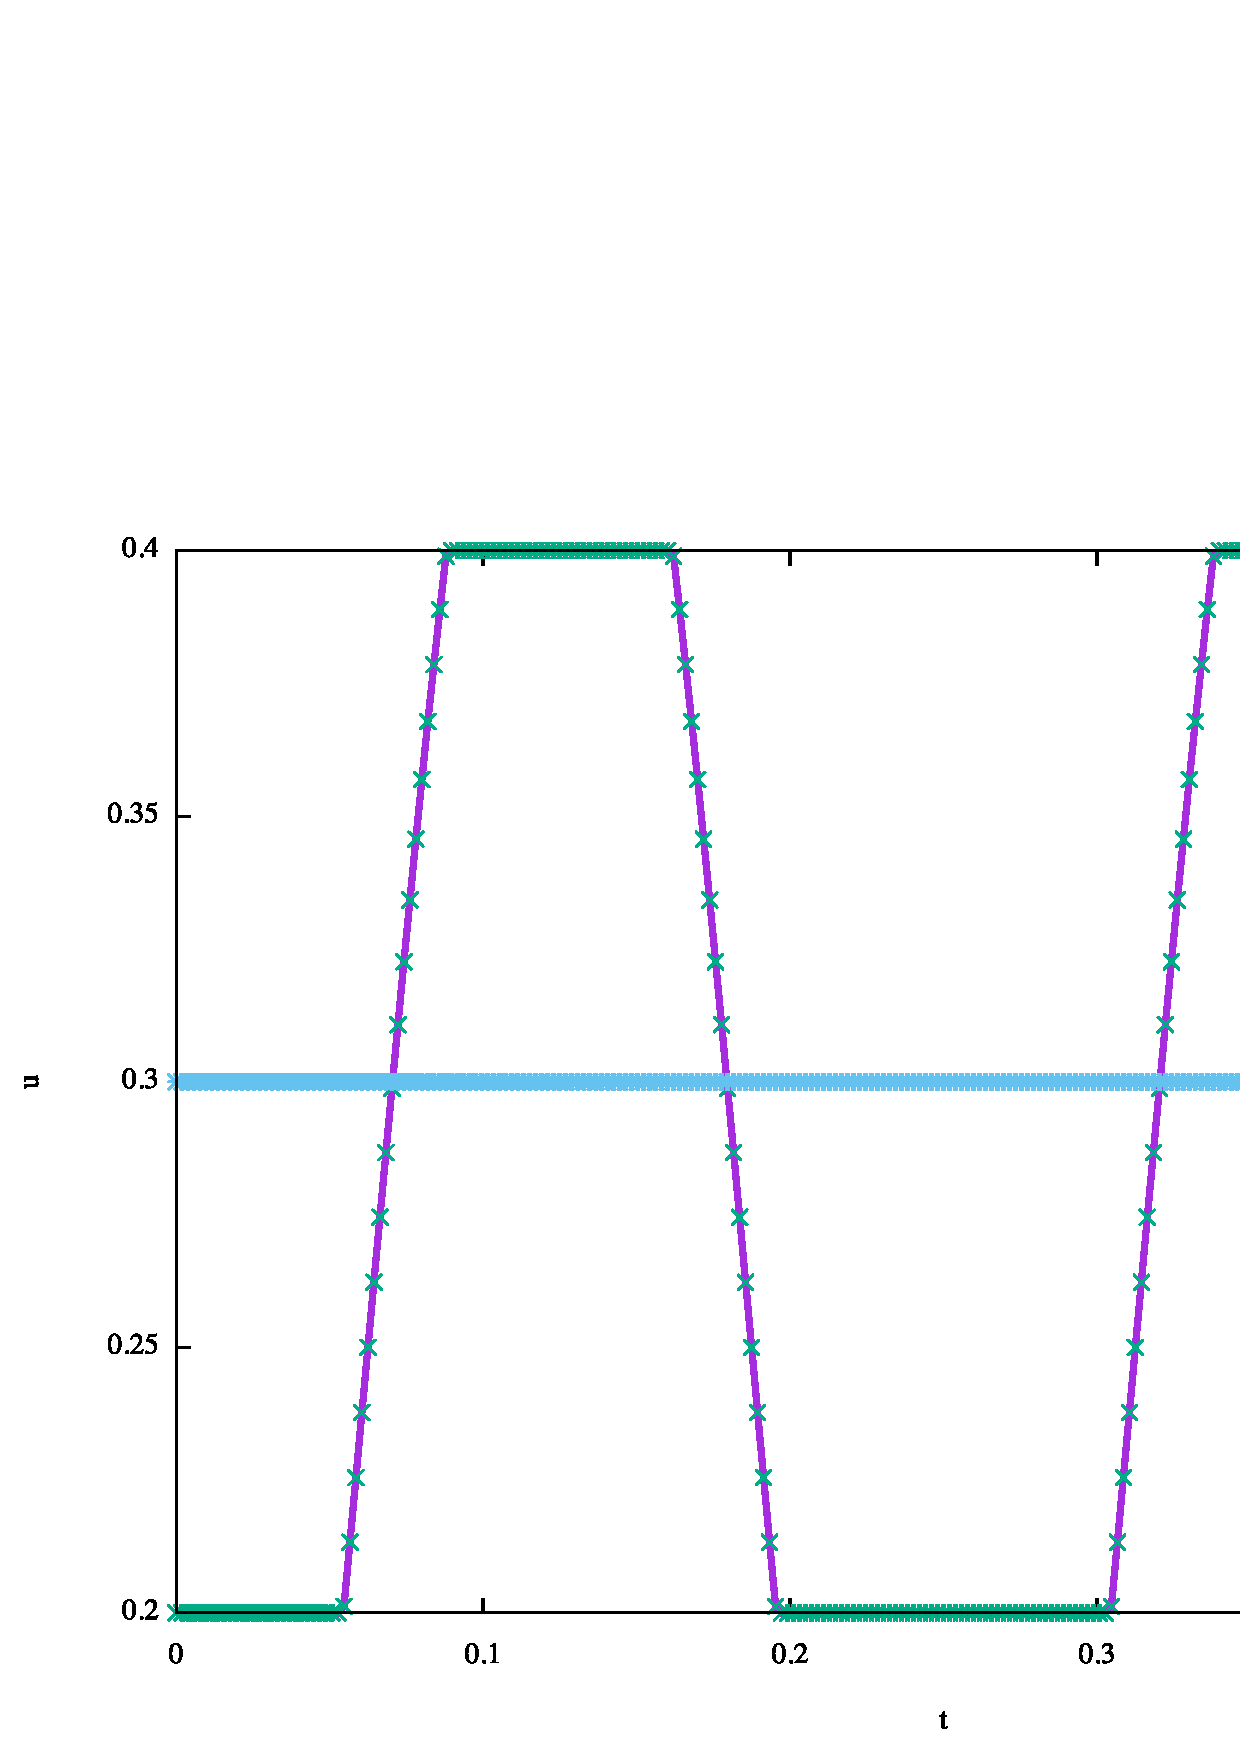
\includegraphics[width=0.2\linewidth]{img/cap6/Imm_PF_02/ControlSol_N150_l8}}
\caption{Test Case 02 $\overline{u}$ e $u_k$ risultati dell'algoritmo di punto fisso}
\label{fig:504}
\end{figure}

\end{frame}

\begin{frame}
\frametitle{Test Case 02 Punto fisso}

\begin{table}
\caption{Punto fisso per Test case II: errori e EOC }
\label{puntofissoII}
\centering

\begin{tabular}{cllll}
\toprule
{l}           &  {$ \norma{\bar{u}-u_{kh}}_{L^2(L^2)} $} &  {$ \norma{\bar{y}-y_{kh}}_{L^2(L^2)} $} &  {$ EOC_{u} $} &  {$ EOC_y $} \\
\midrule
1            &  0.11547 &  0.577323 &  {$-$} &  {$-$} \\
2            &  0.049267 &  0.463462 &  1.66741 &  0.430045 \\
3            &  0.0229418 &  0.136413 &  1.30029 &  2.08074 \\
4            &  0.0036817 &  0.0594452 &  2.87676 &  1.30605 \\
5            &  0.000908002 &  0.0286805 &  2.1105 &  1.09882 \\
6            &  0.000229782  &  0.0142118 &  2.02708 &  1.0358 \\
7            &  0.0000652737 &  0.0070899 &  1.83615 &  1.01455 \\      
8            &  0.0000267529 &  0.003543 &  1.29406 &  1.00643 \\
\bottomrule
\end{tabular}              

\end{table}


\end{frame}

\begin{frame}
\frametitle{Test Case 02 Punto fisso}
\begin{table}
\caption{Punto fisso per Test case II: errori e EOC }
\label{puntofissoIIbis}
\centering

\begin{tabular}{cllll}
\toprule
{l}           &  {$ \norma{\bar{y}-\pi_{P^*_k}y_{kh}}_{L^2(L^2)} $} &  {$ \norma{\bar{p}-p_{kh}}_{L^2(L^2)} $} &  {$ EOC_{\pi y} $} &  {$ EOC_p $} \\
\midrule
1            &  0.408219 &  0.57735 &  {$-$} &  {$-$} \\
2            &  0.428289 &  0.181146 &  0.0939571 &  2.26916 \\
3            &  0.108057  &  0.0846821 &  2.34293 &  1.29366 \\
4            &  0.0223162  &  0.0224906 &  2.48014 &  2.08464 \\
5            &  0.00443799 &  0.00571816 &  2.43498 &  2.06462 \\
6            &  0.000929298 &  0.00145281 &  2.3065 &  2.02122 \\
7            &  0.000203934 &  0.000385864 &  2.21269 &  1.93423 \\      
8            &  0.0000465654 &  0.000130114 &  2.14277 &  1.57715 \\
\bottomrule
\end{tabular}              
\end{table}

\end{frame}

\begin{frame}
\frametitle{Test Case 02 Semi-Newton}
\begin{figure}
\centering%
\subfigure[{l = 1}]%
{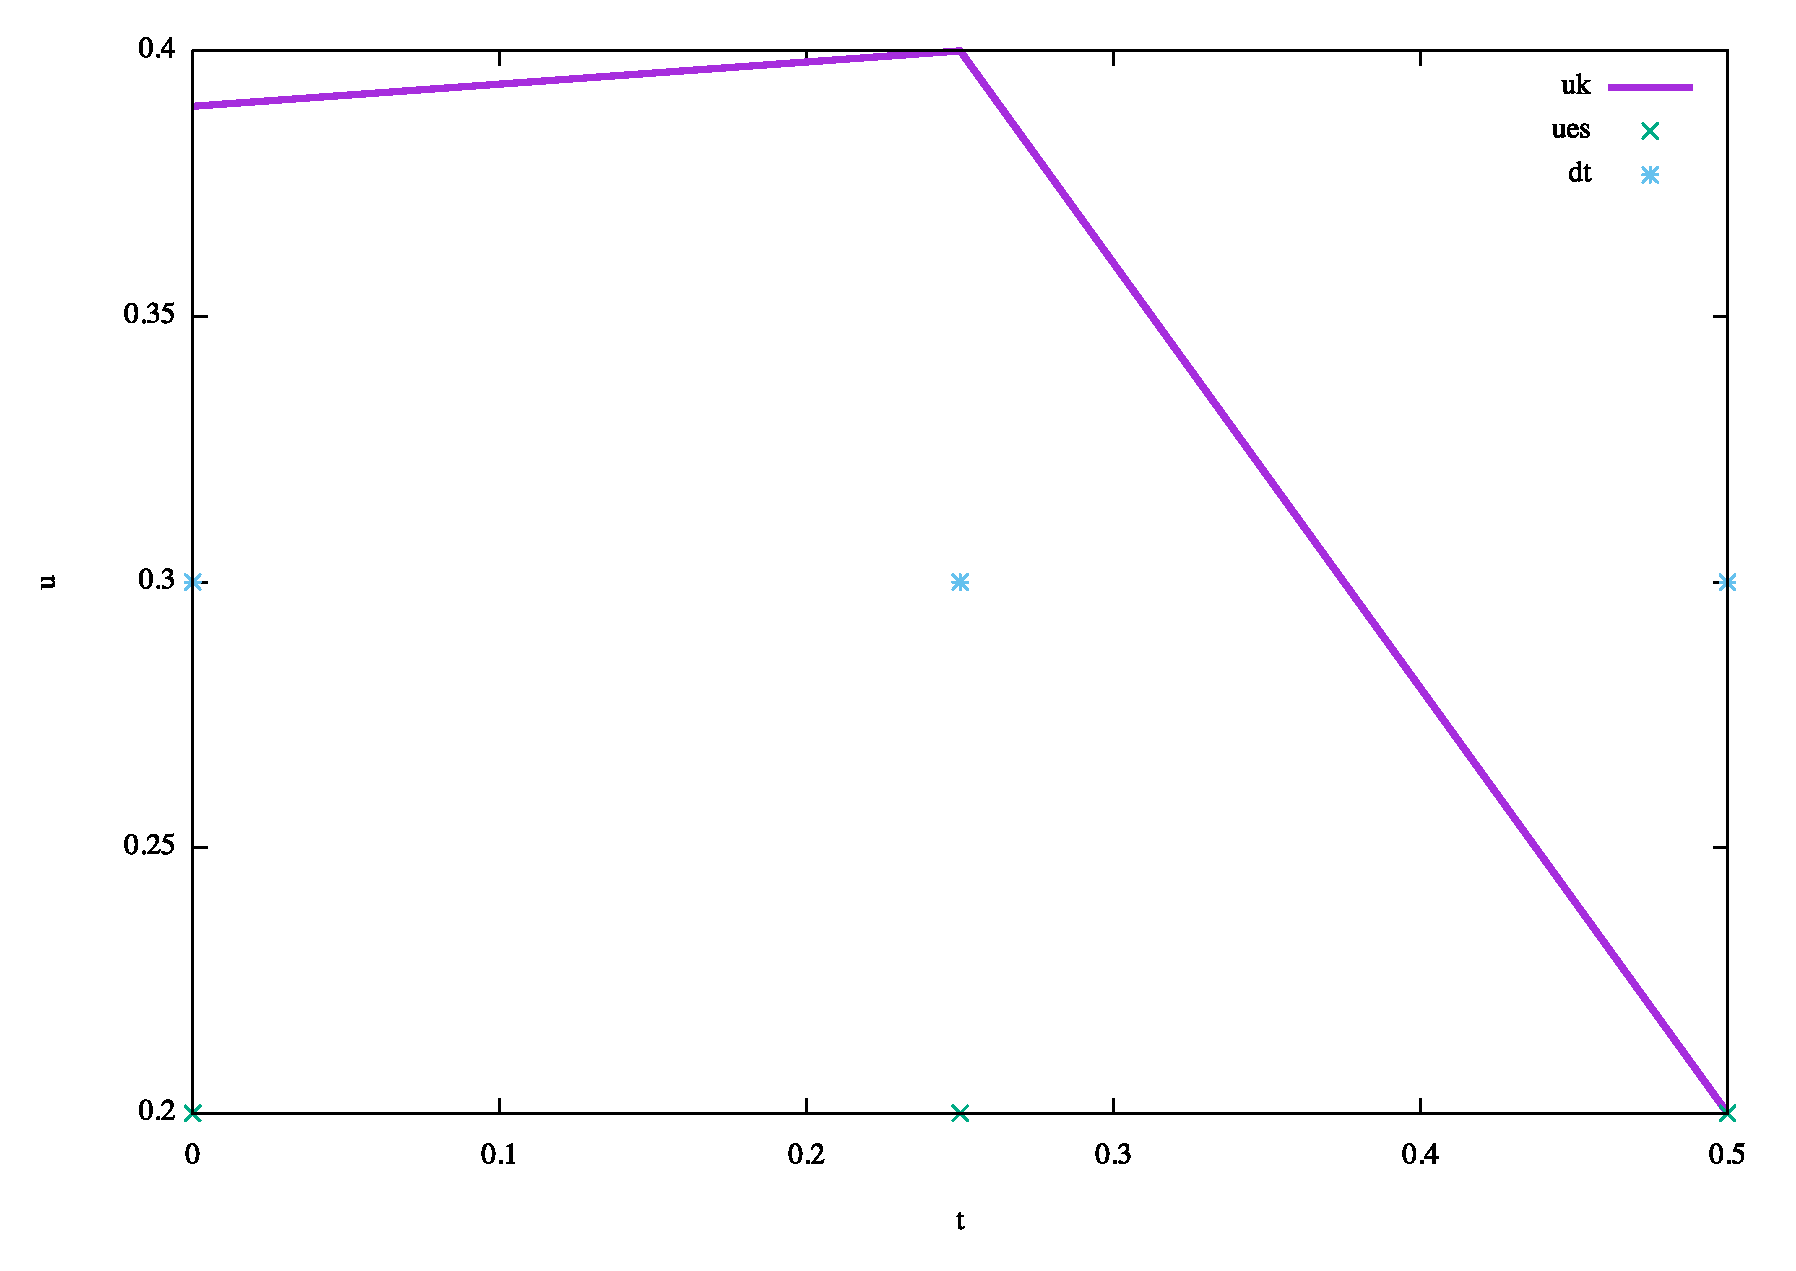
\includegraphics[width=0.2\linewidth]{img/cap6/Imm_CG_02/ControlSol_N150_l1}}\qquad
\subfigure[\protect\url{l = 2}]%
{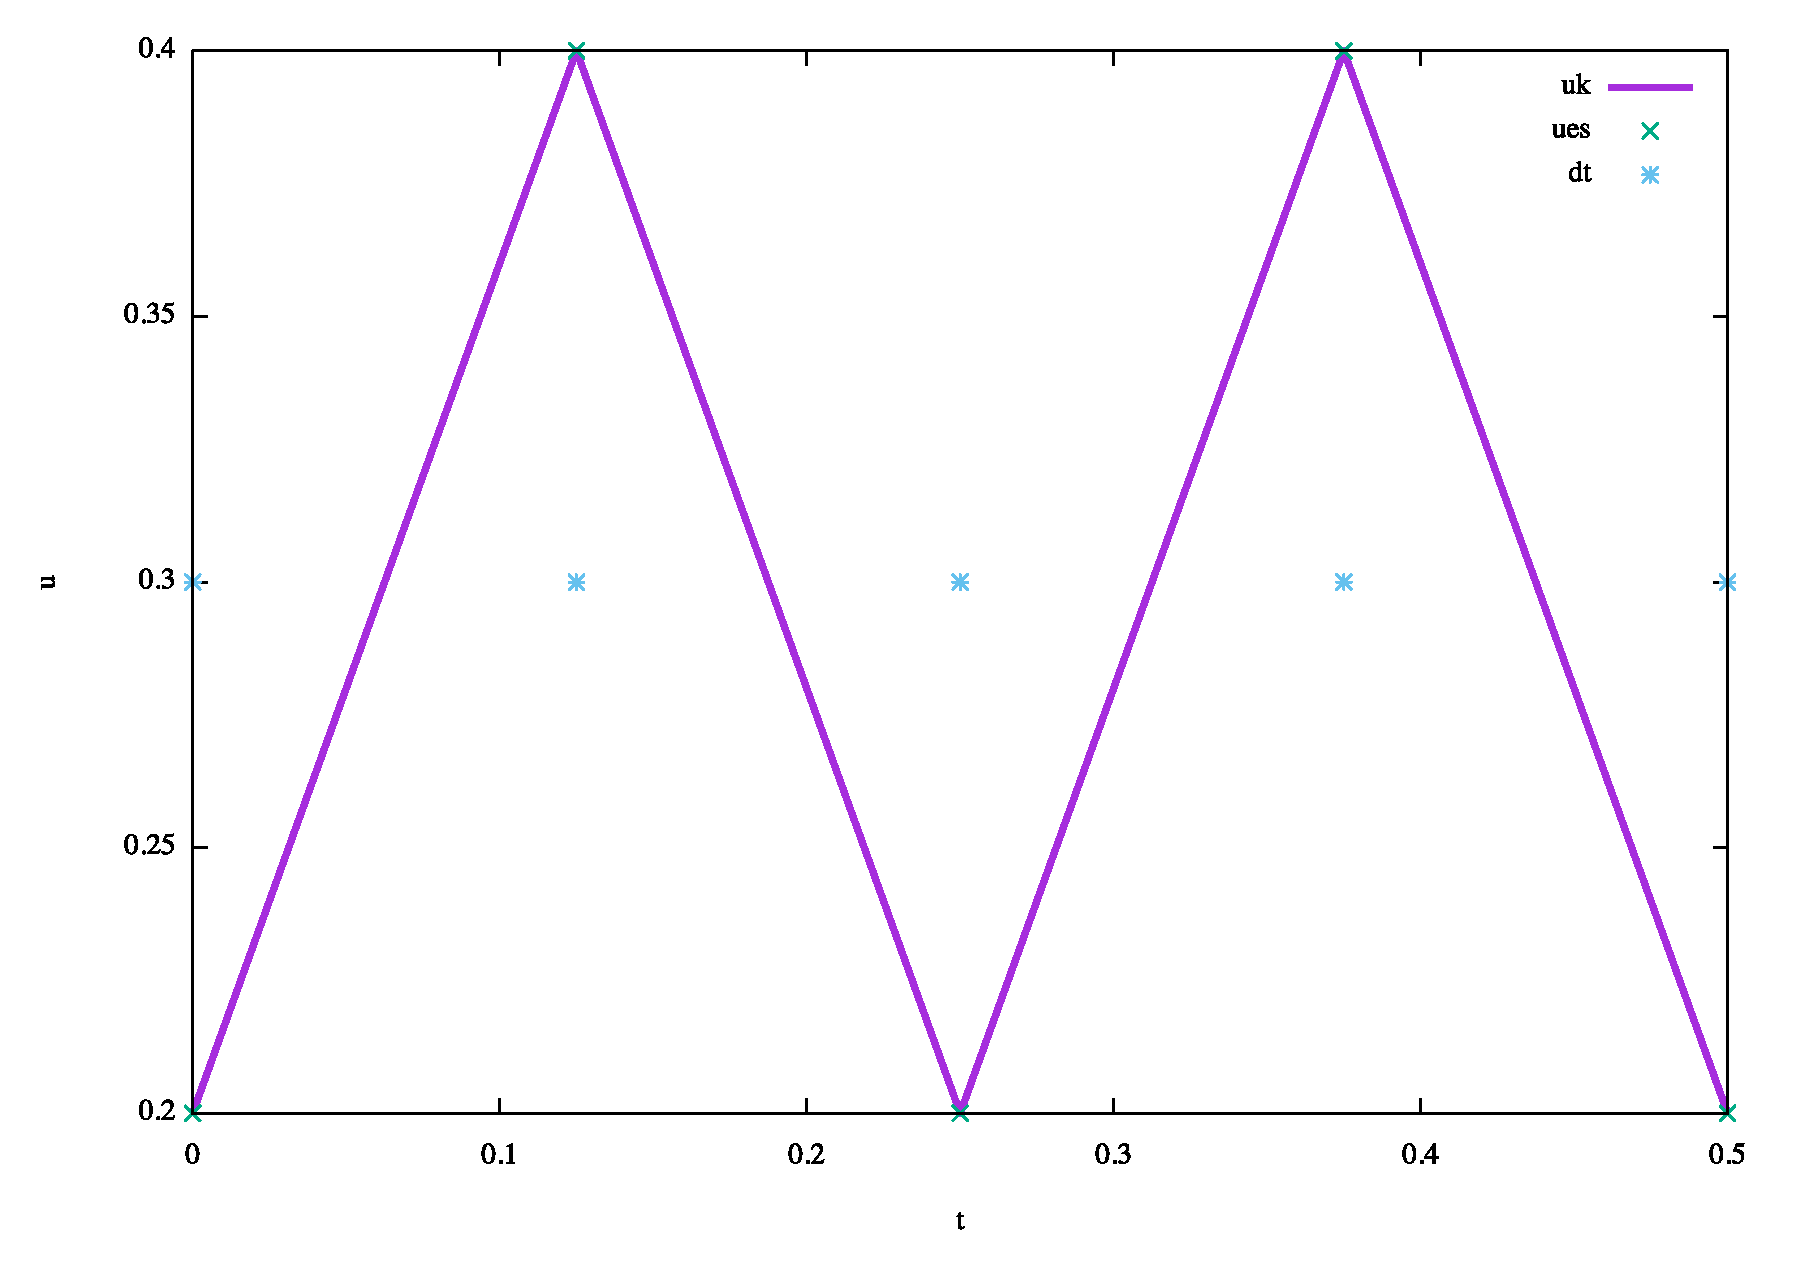
\includegraphics[width=0.2\linewidth]{img/cap6/Imm_CG_02/ControlSol_N150_l2}}\qquad
\subfigure[\protect\url{l = 3}]%
{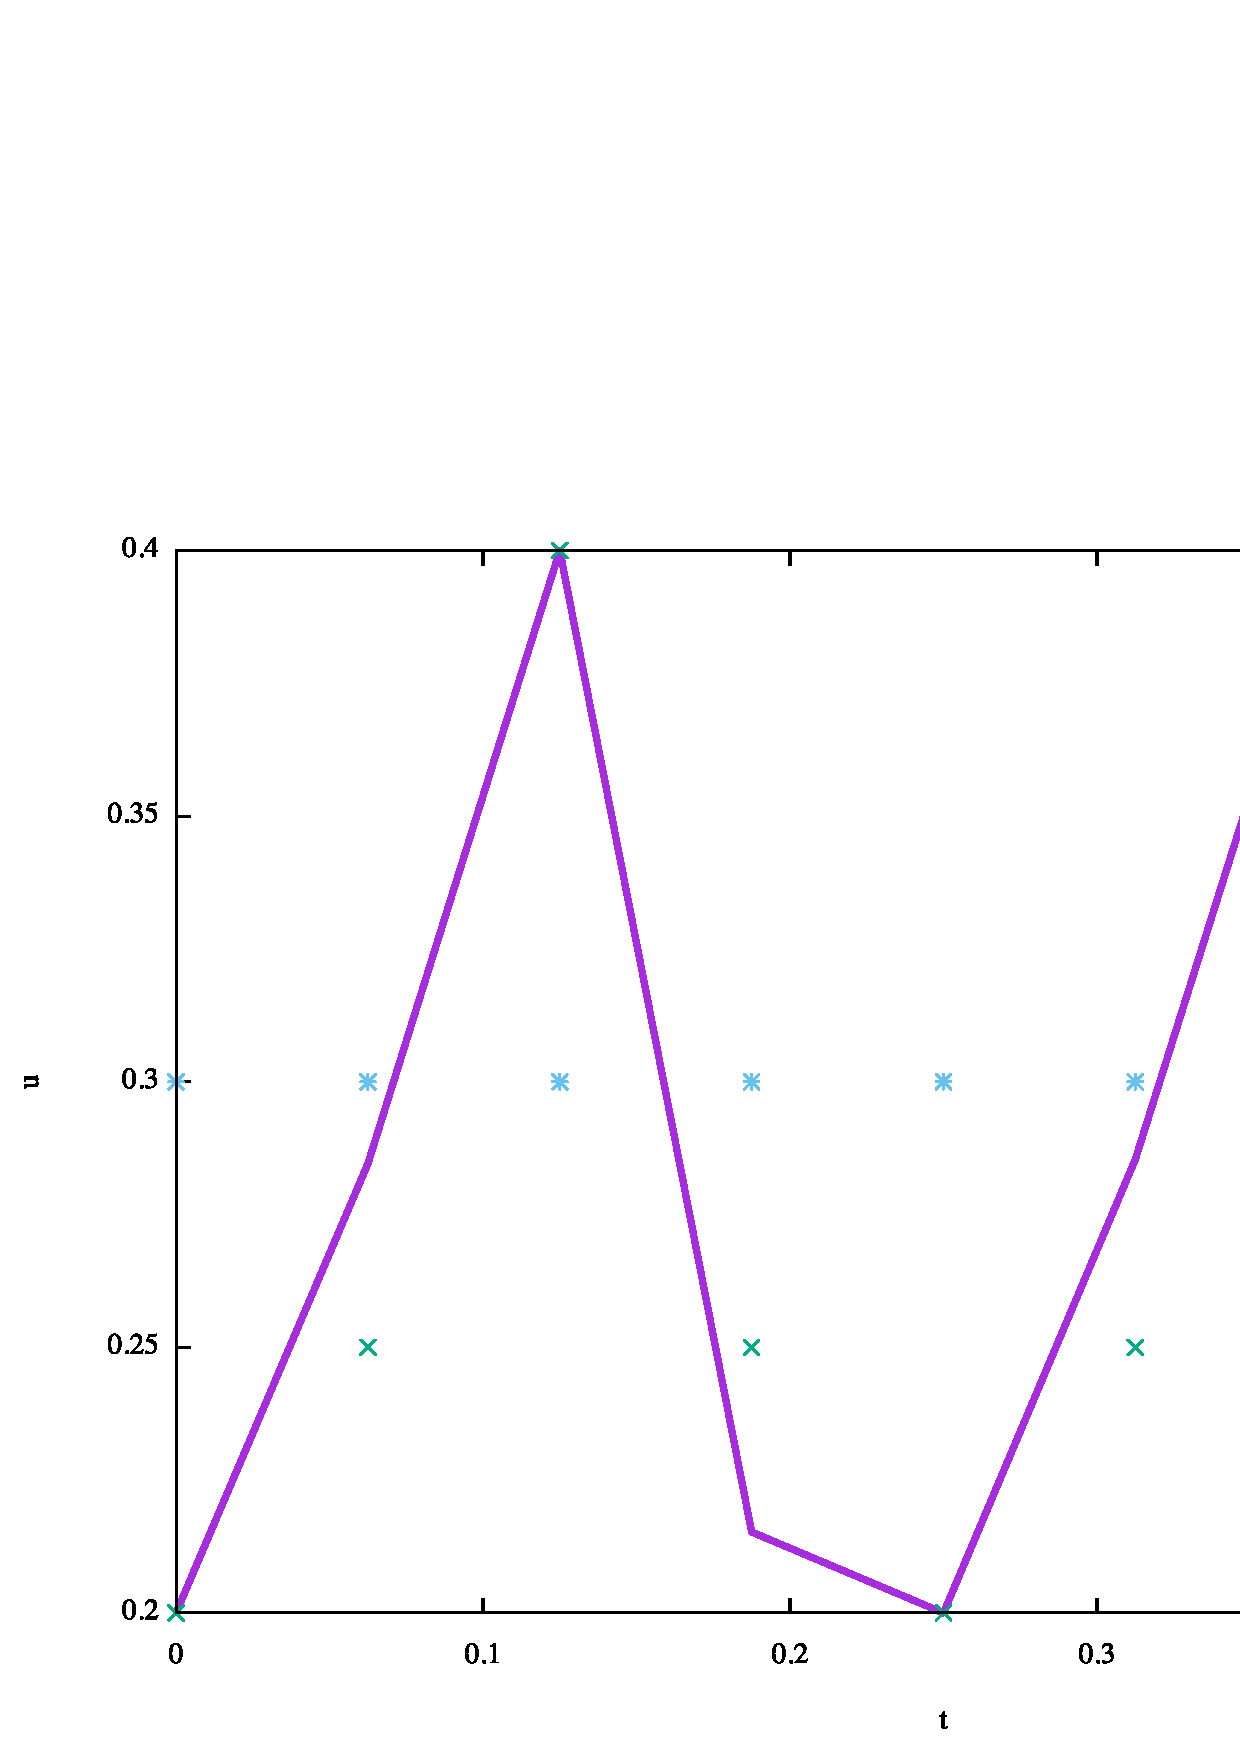
\includegraphics[width=0.2\linewidth]{img/cap6/Imm_CG_02/ControlSol_N150_l3}}\qquad
\subfigure[\protect\url{l = 4}]%
{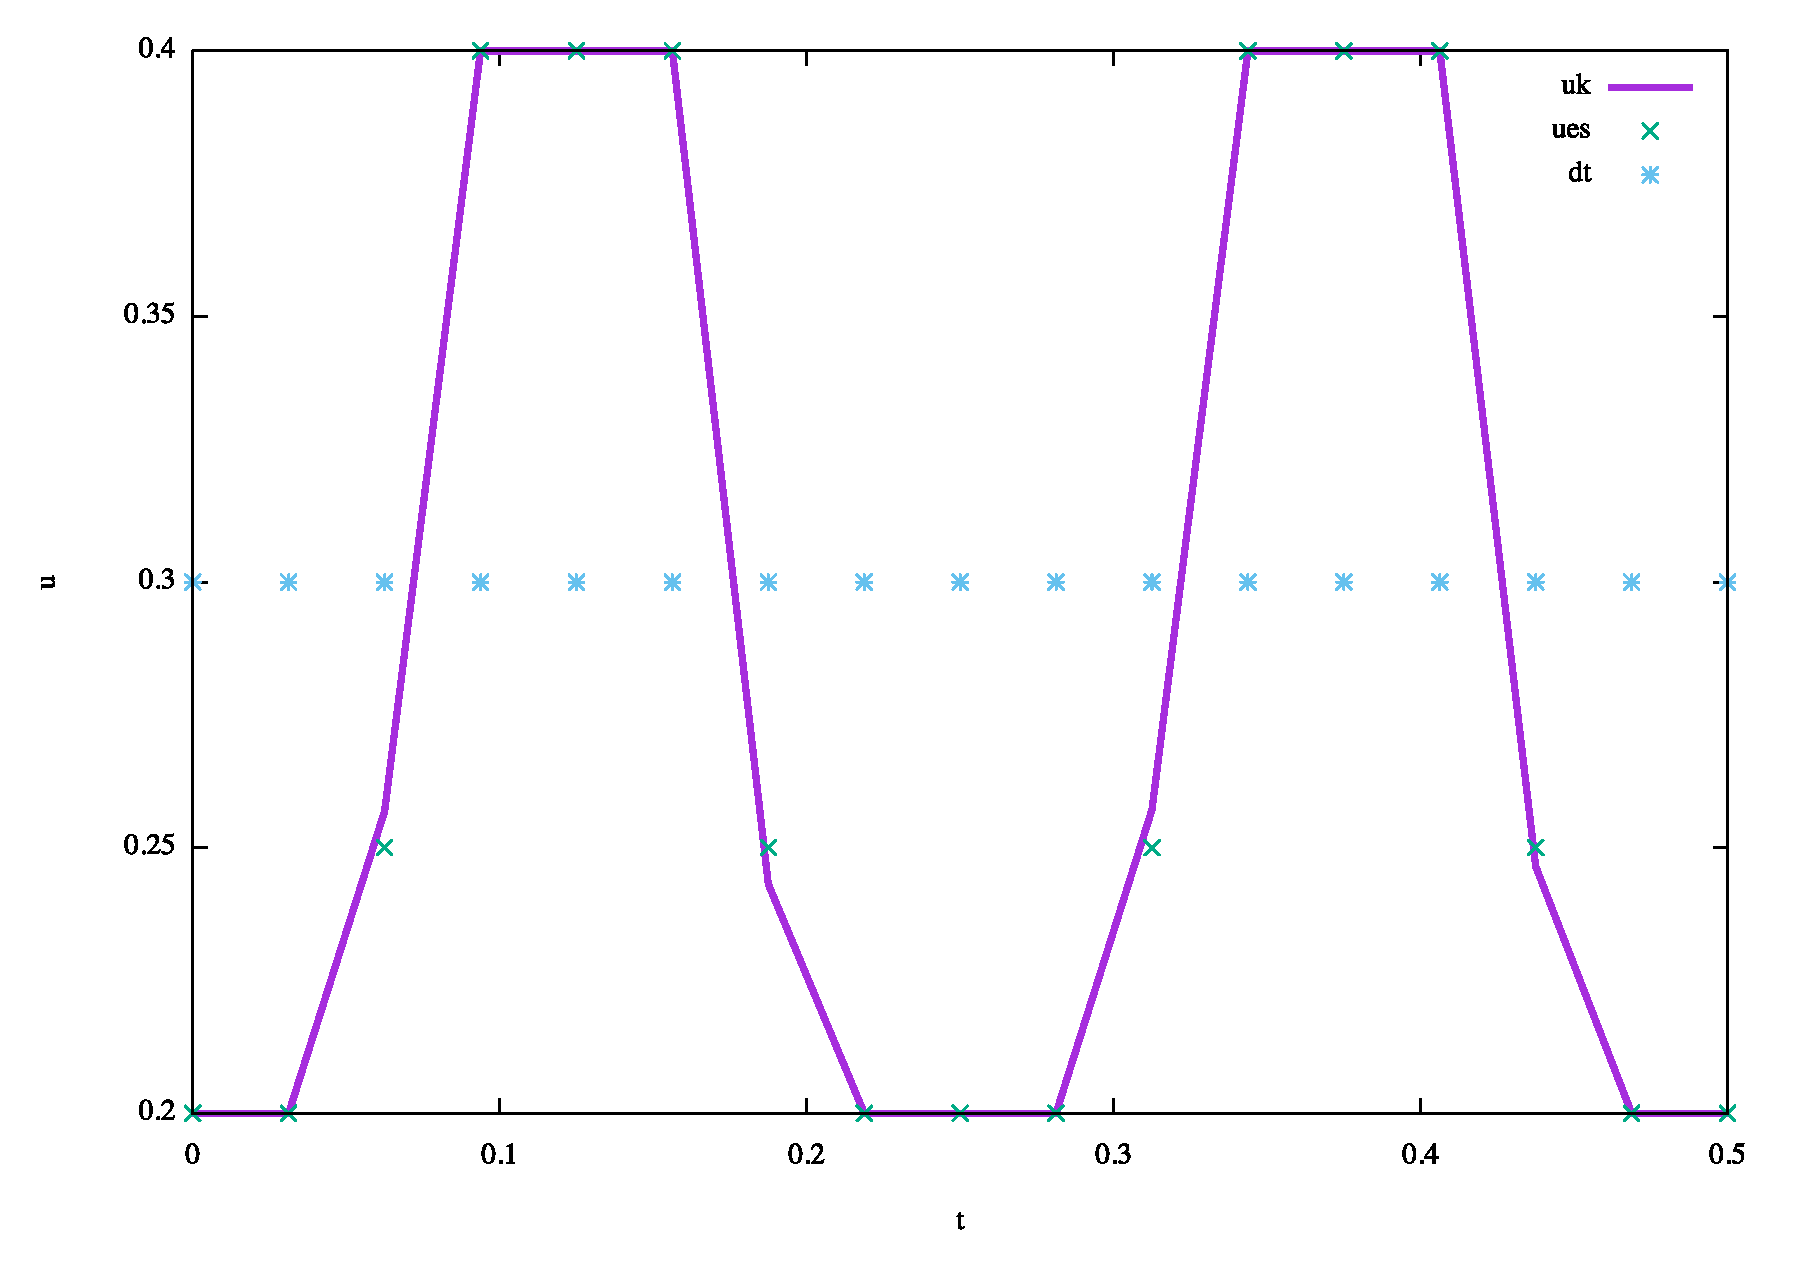
\includegraphics[width=0.2\linewidth]{img/cap6/Imm_CG_02/ControlSol_N150_l4}}\qquad
\subfigure[\protect\url{l = 5}]%
{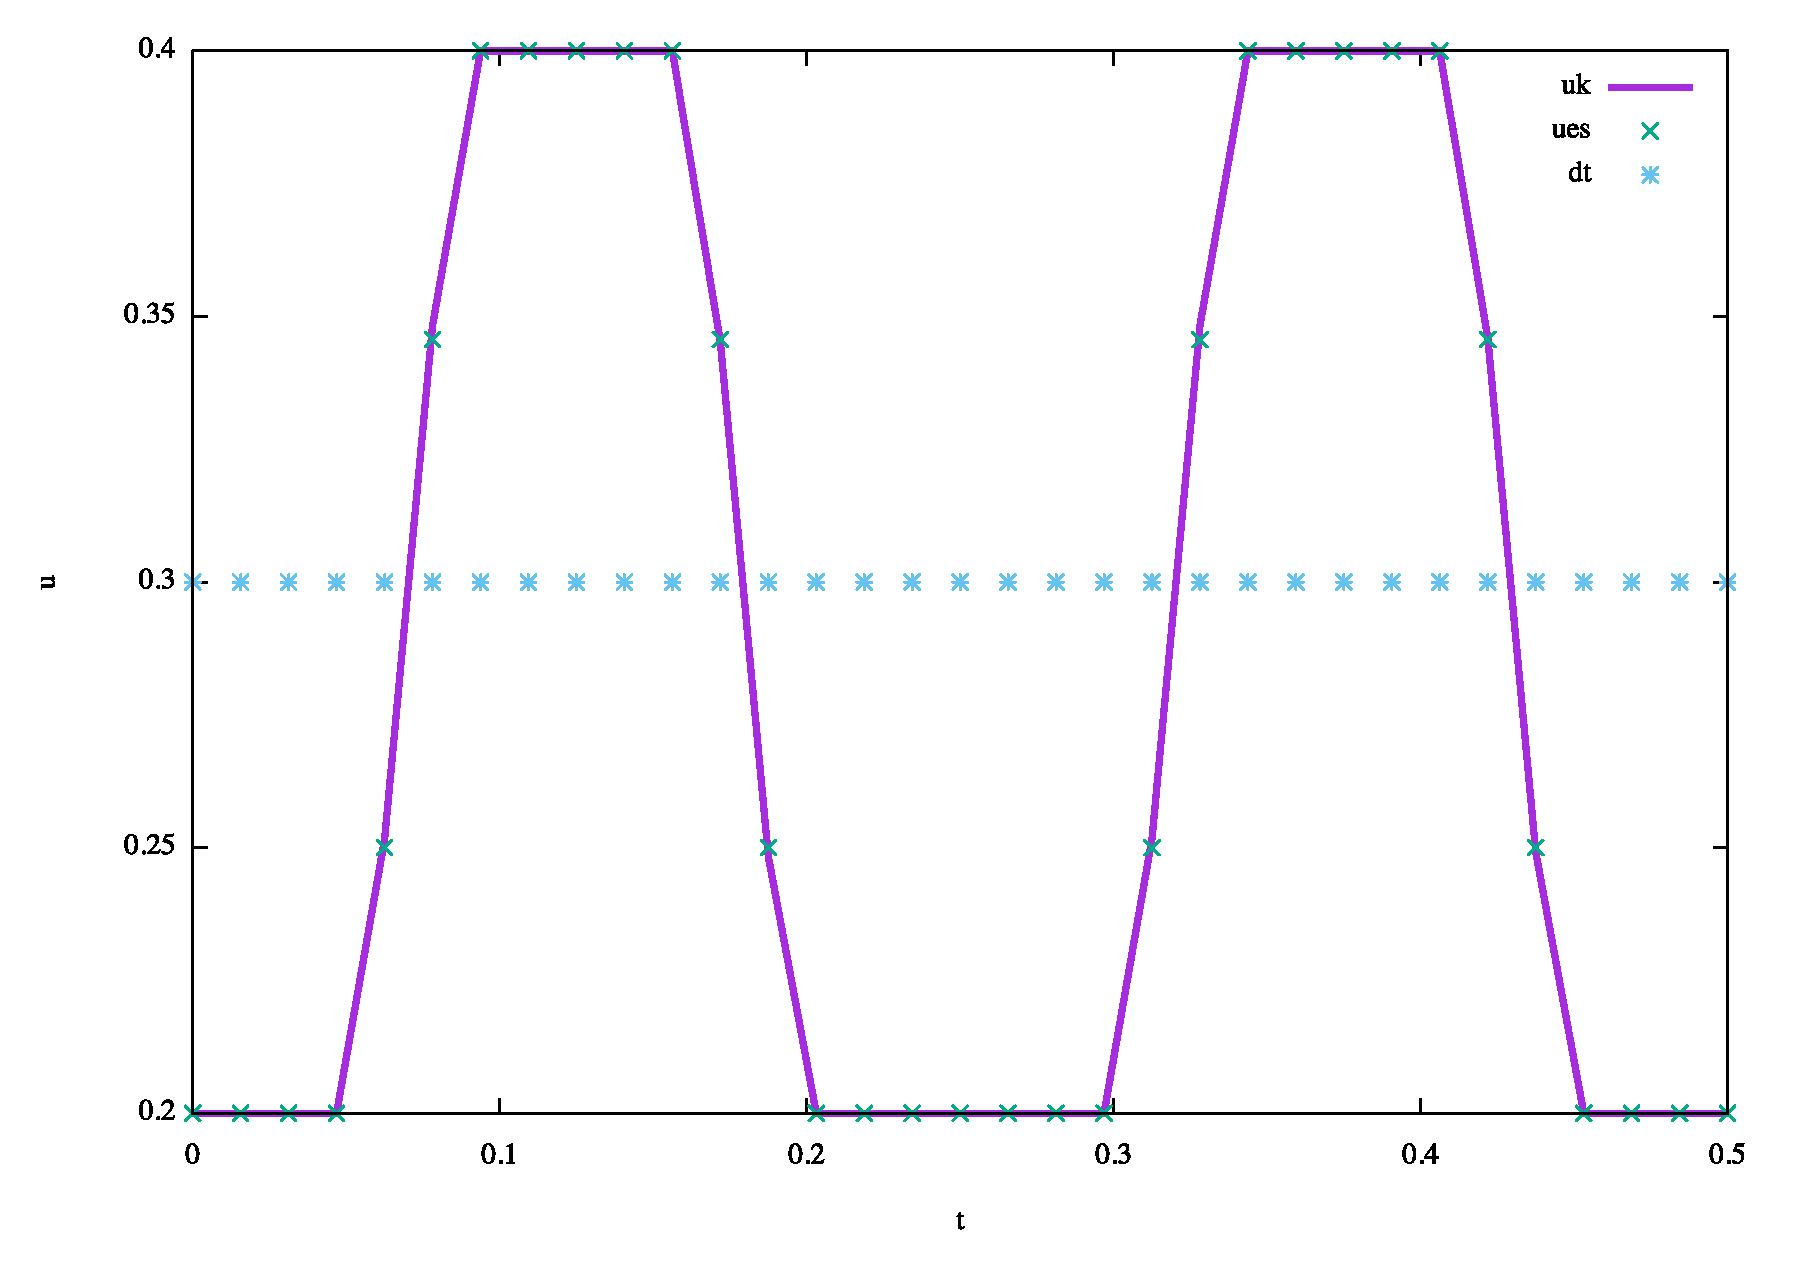
\includegraphics[width=0.2\linewidth]{img/cap6/Imm_CG_02/ControlSol_N150_l5}}\qquad
\subfigure[\protect\url{l = 6}]%
{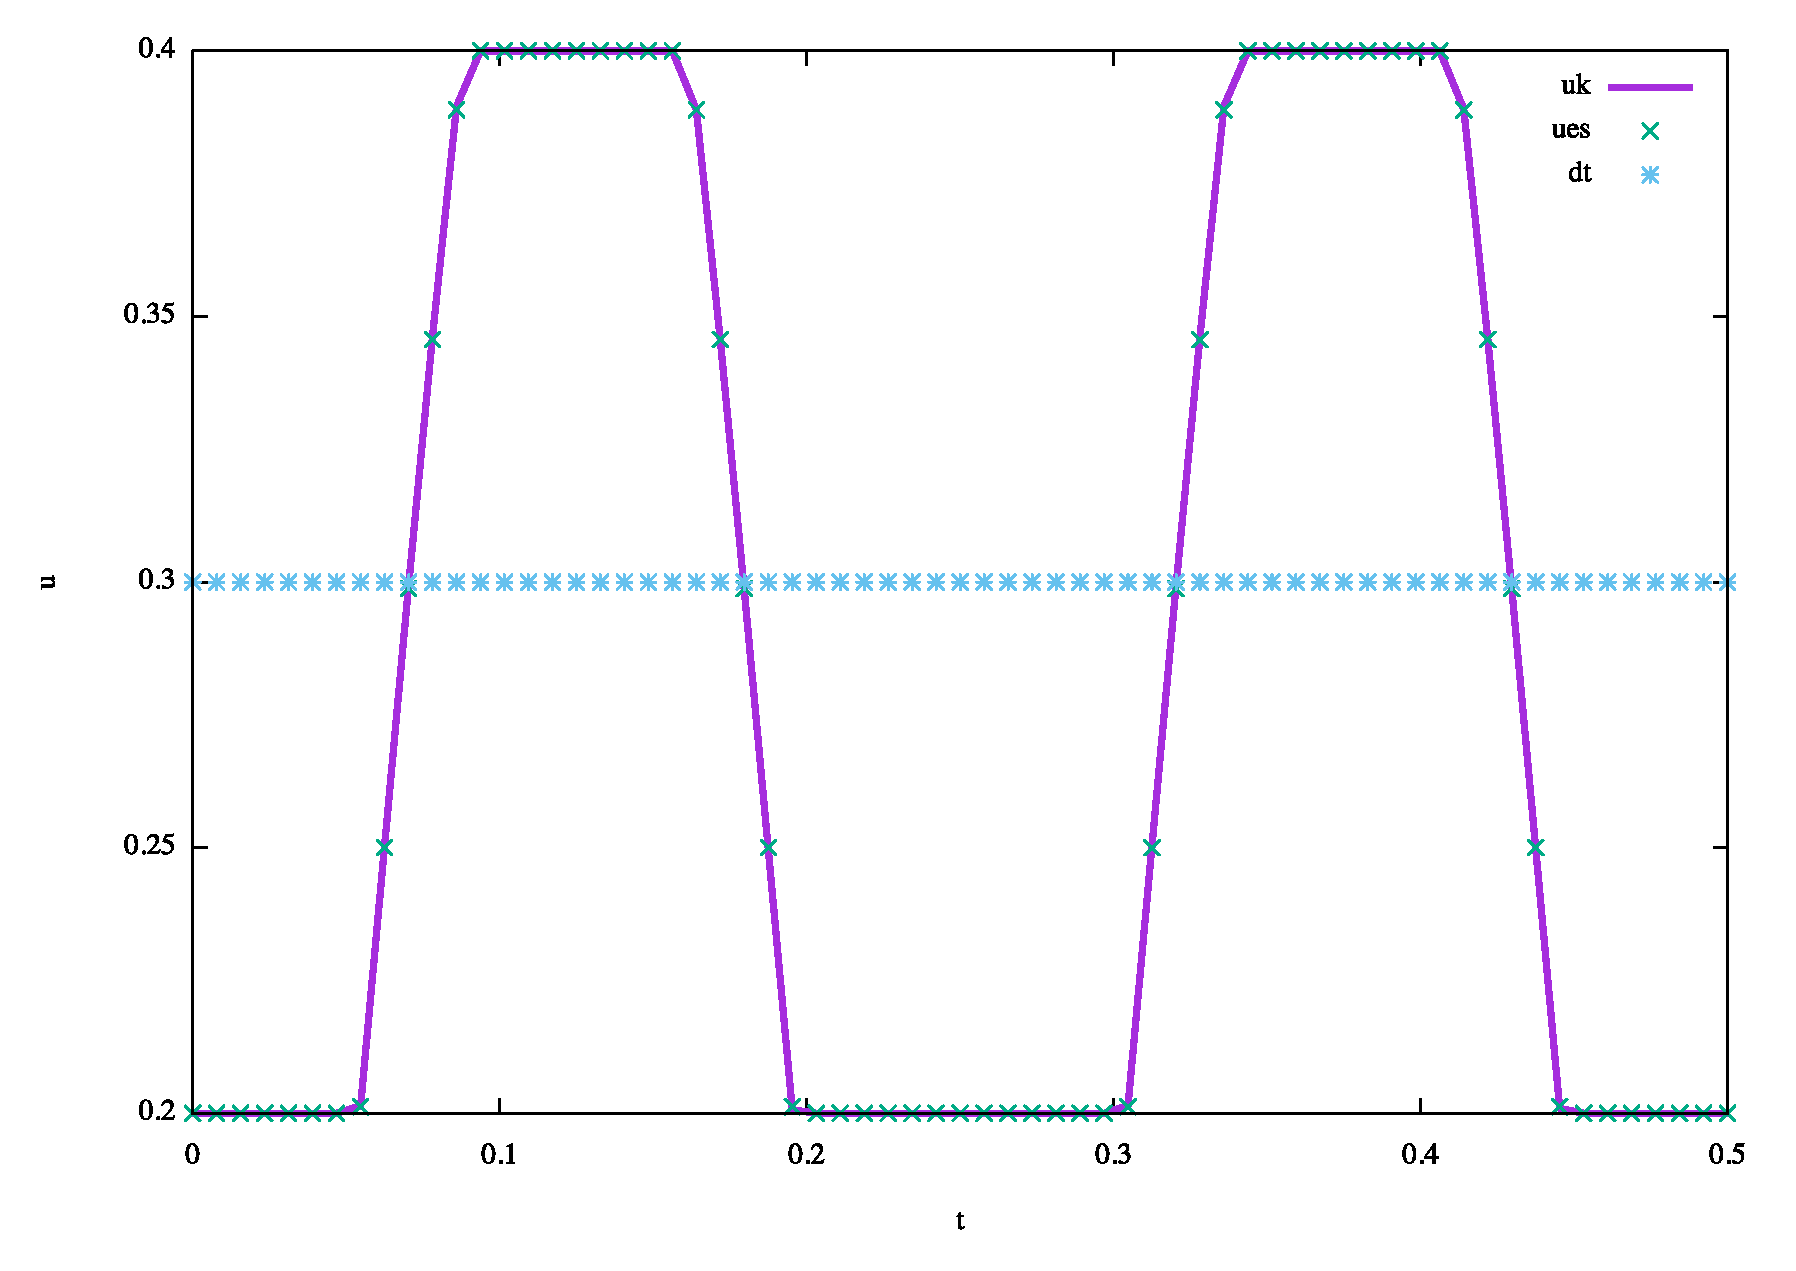
\includegraphics[width=0.2\linewidth]{img/cap6/Imm_CG_02/ControlSol_N150_l6}}\qquad
\subfigure[\protect\url{l = 7}]%
{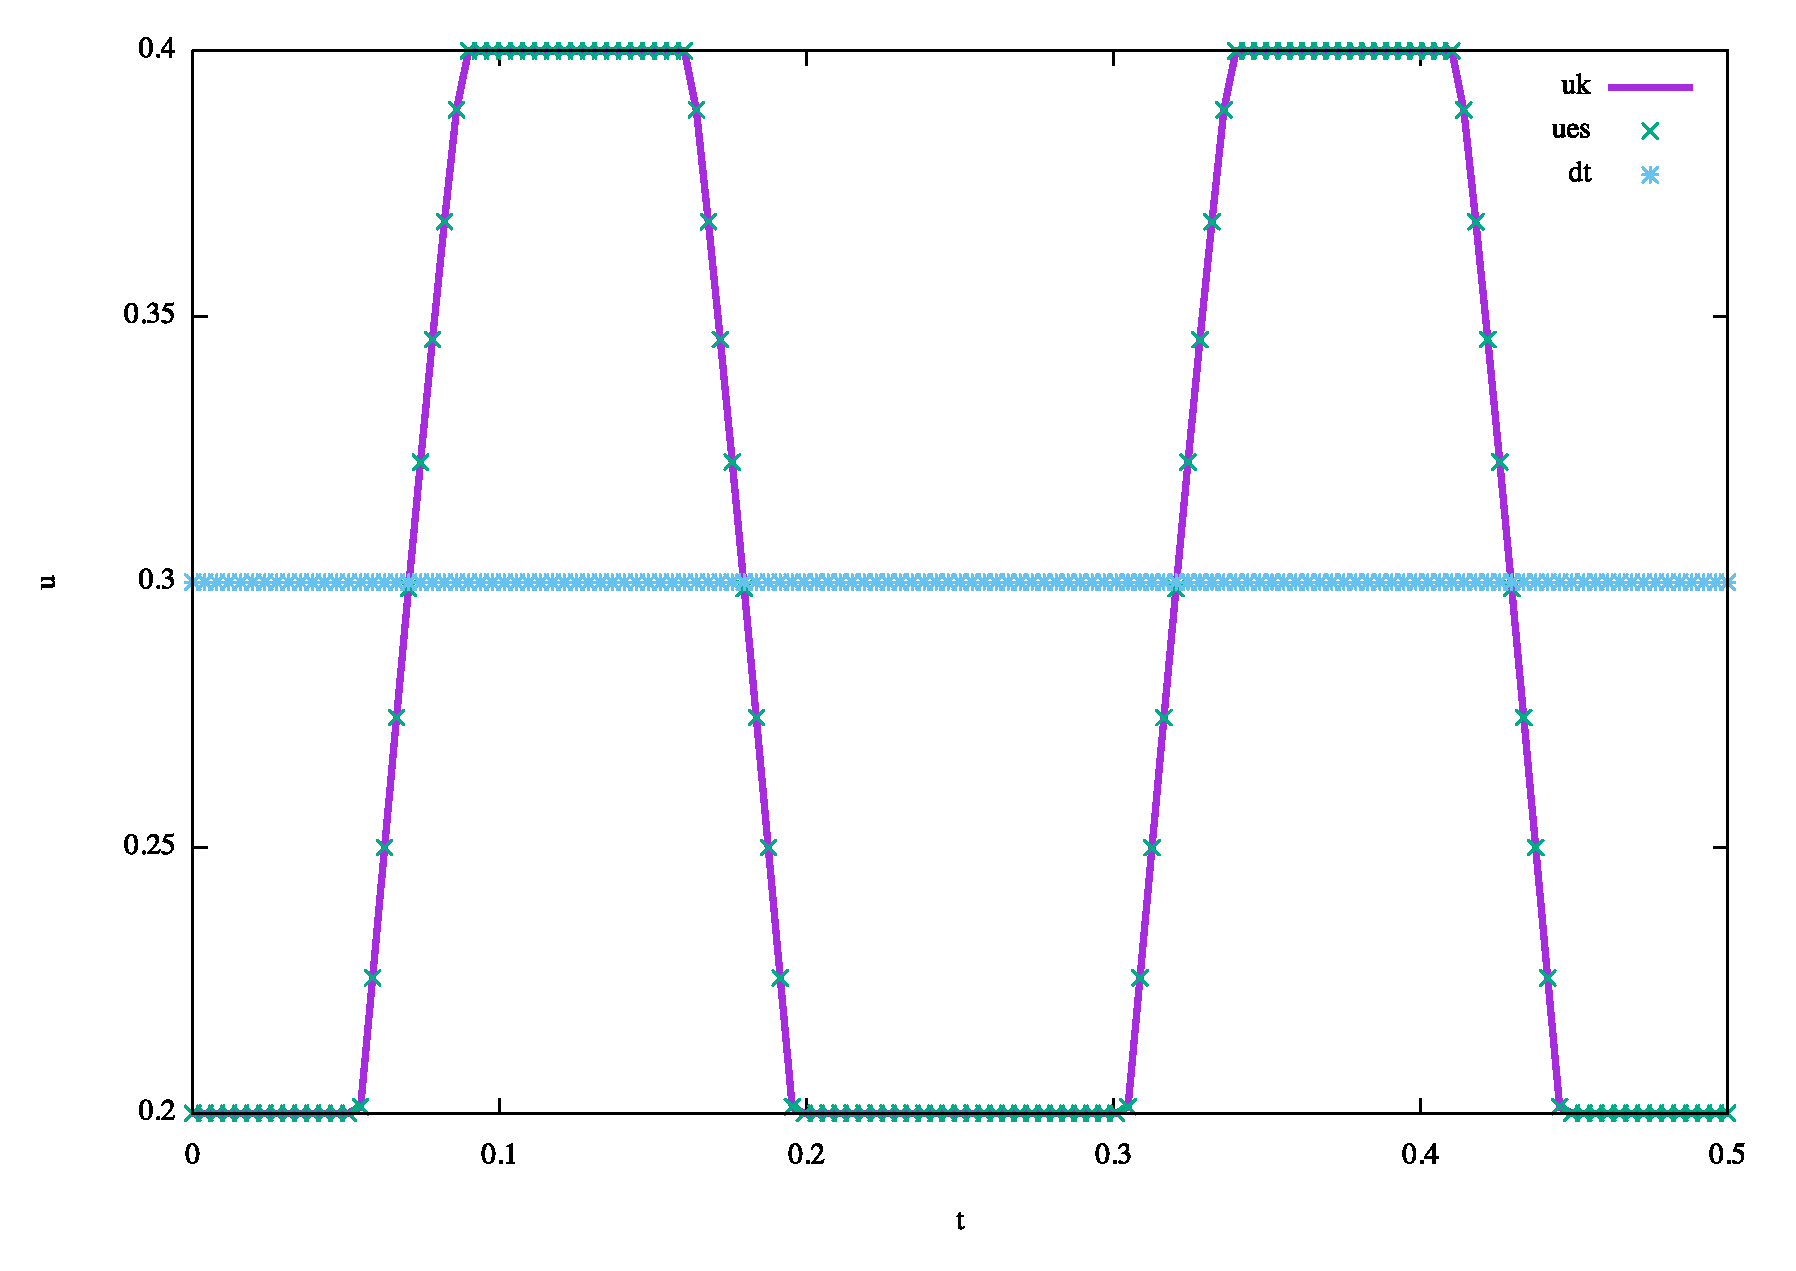
\includegraphics[width=0.2\linewidth]{img/cap6/Imm_CG_02/ControlSol_N150_l7}}\qquad
\subfigure[\protect\url{l = 8}]%
{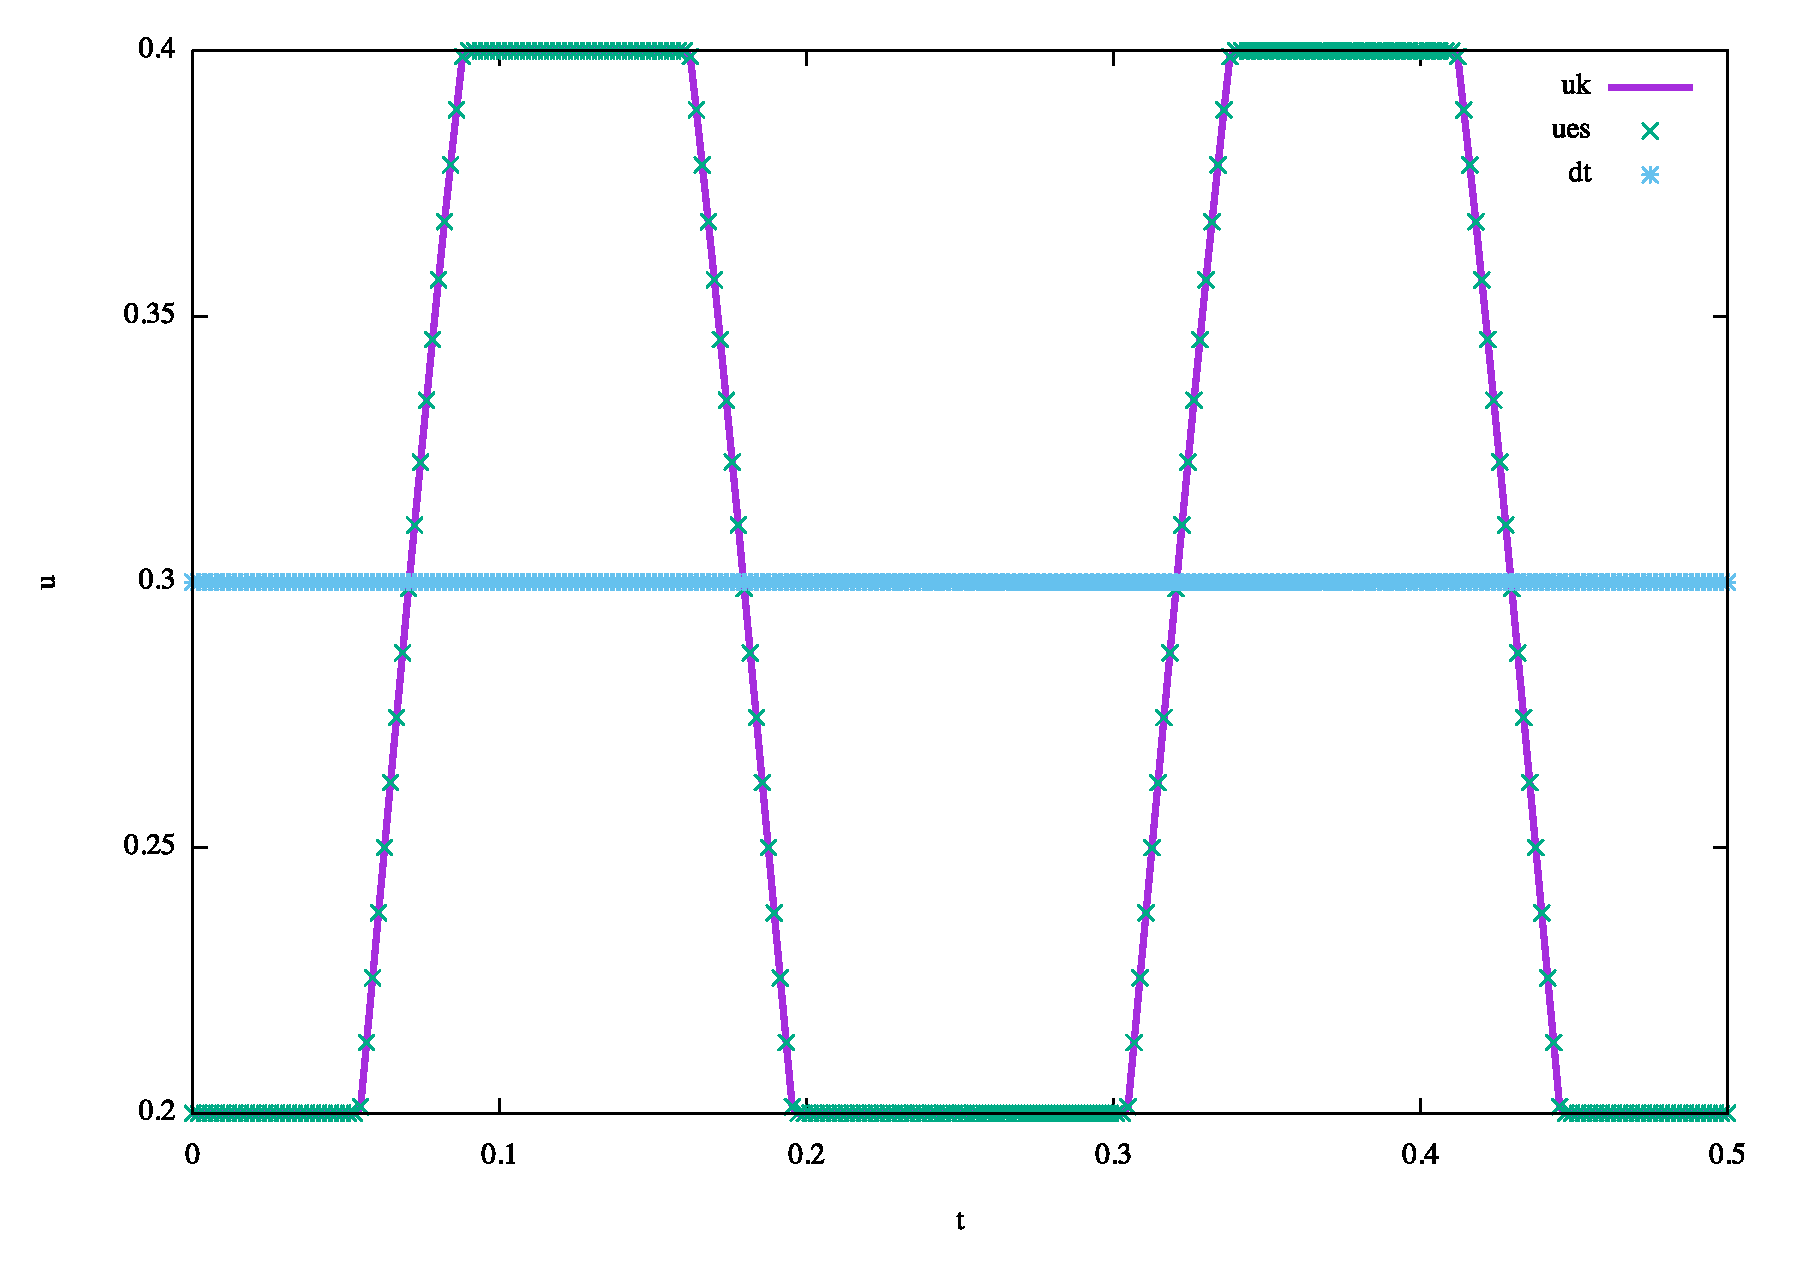
\includegraphics[width=0.2\linewidth]{img/cap6/Imm_CG_02/ControlSol_N150_l8}}
\end{figure}

\end{frame}

\begin{frame}
\frametitle{Test Case 02 Semi-Newton}
\begin{table}
\caption{Newton per Test case II: errori e EOC }
\label{newtonII}
\centering

\begin{tabular}{cllll}
\toprule
{l} &  {$ \norma{\bar{u}-u_{kh}}_{L^2(L^2)} $} &  {$ \norma{\bar{y}-y_{kh}}_{L^2(L^2)} $} &  {$ EOC_{u} $} &  {$ EOC_y $} \\
\midrule
1            &  0.115495 &  0.579976 &  {$-$} &  {$-$} \\
2            &  0.076157  &  0.462076 &  0.815213 &  0.444884 \\
3            &  0.0127336  &  0.136402 &  3.04286 &  2.07579 \\
4            &  0.00222359 &  0.0594457 &  2.74395 &  1.30591 \\
5            &  0.000541362 &  0.0286803 &  2.12996 &  1.09884 \\
6            &  0.000138463  &  0.0142117 &  2.01139 &  1.03579 \\
7            &  0.0000349821 &  0.0070899 &  2.00717 &  1.01455 \\      
8            &  0.0000178053 &  0.003543 &  0.979797  &  1.00643 \\
\bottomrule
\end{tabular}              

\end{table}
\end{frame}

\begin{frame}
\frametitle{Test Case 02 Semi-Newton}
\begin{table}
\caption{Newton per Test case II: errori e EOC }
\label{newtonIIbis}
\centering

\begin{tabular}{cllll}
\toprule
{l}  &  {$ \norma{\bar{y}-\pi_{P^*_k}y_{kh}}_{L^2(L^2)} $}  &  {$ \norma{\bar{p}-p_{kh}}_{L^2(L^2)} $}        &  {$ EOC_{\pi y} $} &  {$ EOC_p $} \\
\midrule
1 			 &  0.410488 &  0.57748 &  {$-$} & {$-$} \\
2            &  0.427682 &  0.181205 &  0.080328 &  2.26897 \\
3            &  0.108041 &  0.0846824 &  2.34076 &  1.29421 \\
4            &  0.0223131  &  0.0224907 &  2.48014 &  2.08463 \\
5            &  0.00443687 &  0.00571824 &  2.43516  &  2.06461 \\
6            &  0.0009289  &  0.00145285 &  2.30675 &  2.02121 \\
7            &  0.000203852 &  0.000385873 &  2.21265 &  1.93423 \\      
8            &  0.0000465544 &  0.000130118 &  2.14254 &  1.57714 \\
\bottomrule
\end{tabular}              

\end{table}

\end{frame}


\section{Conclusioni}
\begin{frame}
Entrambi gli algoritmi implementati confermano i risultati teorici per l'ordine di convergenza dell'errore nei problemi di controllo ottimo parabolico se viene utilizzato uno schema di Petrov Galerkin.
Per il primo test case, nel quale $\alpha$ è minore, il metodo di Newton converge più velocemente che quello di punto fisso.

Possibili lavori futuri:
\begin{enumerate}
\item analisi analitica di semi-Newton nel caso per i problemi di controllo ottimo parabolici
\item scrittura/lettura su/da file per le soluzioni dei problemi di stato ed aggiunto
%\item spazi EF su $\Omega$ differenti per il problema di stato e quello di aggiunto nel caso dell'algoritmo di Semi-Newton
\end{enumerate}

\end{frame}

\begin{frame}
\centering
Grazie Per L'Attenzione
\end{frame}

\begin{frame}
APPENDICE
\end{frame}

\begin{frame}
\frametitle{Test Case 01 dati del problema}
\begin{tabular}{|c|c|}
\hline
\textbf{funzione} & \textbf{TestCase01}\\
\hline
$g_1(x_1,x_2)$ & $sin({\pi}x_1)sin({\pi}x_2)$\\
\hline
$g_0(t,x_1,x_2)$ & $ -{\pi}^2w_a(t,x_1,x_2) - BP_{U_{ad}} \left( -\frac{1}{4\alpha} (e^{a{\pi}^2t} - e^{a{\pi}^2T}) \right)$ \\
\hline
$w_a(t,x_1,x_2)$ & $e^{a{\pi}^2t}sin({\pi}x_1)sin({\pi}x_2) \text{, } a \in \mathbb{R}$ \\
\hline
$y_d(t,x_1,x_2)$ & $\frac{a^2 - 5}{2 + a}{\pi}^2w_a(t,x_1,x_2) + 2{\pi}^2w_a(T,x_1,x_2)$ \\
\hline
$y_0(x_1,x_2)$ & $\frac{- 1}{2 + a}{\pi}^2w_a(0,x_1,x_2)$ \\
\hline
$\overline{u}(t,x_1,x_2)$ & $P_{U_{ad}} \left( -\frac{1}{4\alpha}(e^{a{\pi}^2t}-e^{a{\pi}^2T} \right)$ \\
\hline
$\overline{y}(t,x_1,x_2)$ & $\frac{- 1}{2 + a}{\pi}^2w_a(0,x_1,x_2)$ \\
\hline
$\overline{p}(t,x_1,x_2)$ & $w_a(t,x_1,x_2) - w_a(T,x_1,x_2)$ \\
\hline
\end{tabular}

\end{frame}

\begin{frame}
\frametitle{Test Case 02 dati del problema}
\begin{tabular}{|c|c|}
\hline
\textbf{funzione} & \textbf{TestCase01}\\
\hline
$g_1(x_1,x_2)$ & $sin({\pi}x_1)sin({\pi}x_2)$\\
\hline
$g_0(t,x_1,x_2)$ & $g_1(x_1,x_2) 2\pi \left( -\frac{a}{T}sin\left( \frac{t}{T}2{\pi}a \right) + \pi cos\left( \frac{t}{T}2{\pi}a \right) \right) - B\overline{u}$ \\
\hline
$w_a(t,x_1,x_2)$ & $cos \left( \frac{t}{T}2{\pi}a \right) \cdot g_1(t,x_1,x_2)$ \\
\hline
$y_d(t,x_1,x_2)$ & $g_1\left( cos\left( \frac{t}{T}2{\pi}a \right)(1-2{\pi}^2) -\frac{2{\pi}a}{T}sin\left( \frac{t}{T}2{\pi}a \right) +2{\pi}^2cos(2{\pi}a) \right)$ \\
\hline
$y_0(x_1,x_2)$ & $g_1(x_1,x_2)$ \\
\hline
$\overline{u}(t,x_1,x_2)$ & $P_{U_{ad}} \left( -\frac{1}{4\alpha}cos \left( \frac{t}{T}2{\pi}a \right) +\frac{1}{4\alpha} \right)$ \\
\hline
$\overline{y}(t,x_1,x_2)$ & $\frac{- 1}{2 + a}{\pi}^2w_a(0,x_1,x_2)$ \\
\hline
$\overline{p}(t,x_1,x_2)$ & $w_a(t,x_1,x_2) - w_a(T,x_1,x_2)$ \\
\hline
\end{tabular}

\end{frame}

\end{document}